\documentclass[11pt]{article}

\usepackage[utf8]{inputenc}
\usepackage[T1]{fontenc}
\usepackage[margin=1.1in]{geometry}
\usepackage{amsmath,amssymb,amsthm}
\usepackage{mathtools}
\usepackage{enumitem}
\usepackage{tikz}
\usetikzlibrary{arrows.meta,positioning,decorations.pathreplacing,calc}
\usepackage[hidelinks]{hyperref}
\usepackage{xcolor}

% Todo macro for placeholders to be filled in later phases.
\newcommand{\todo}[1]{{\color{red}\textbf{[TODO: #1]}}}

% Theorem environments.
\newtheorem{theorem}{Theorem}[section]
\newtheorem{proposition}[theorem]{Proposition}
\newtheorem{lemma}[theorem]{Lemma}
\newtheorem{corollary}[theorem]{Corollary}

\theoremstyle{definition}
\newtheorem{definition}[theorem]{Definition}
\newtheorem{example}[theorem]{Example}

\theoremstyle{remark}
\newtheorem{remark}[theorem]{Remark}
\newtheorem{notation}[theorem]{Notation}

% Notation macros.
\newcommand{\Kp}{\mathrm{Kp}}
\newcommand{\NT}{\mathrm{NT}}
\newcommand{\Sing}{\mathrm{Sing}}
\newcommand{\Chain}{\mathrm{Chain}}
\newcommand{\MB}{\mathrm{MB}}
\newcommand{\TM}{\mathrm{TM}}
\newcommand{\KK}{\mathbb{K}}
\newcommand{\Z}{\mathbb{Z}}
\newcommand{\Zn}{\Z_{\geq 0}}
\newcommand{\g}{\mathfrak{g}}
\newcommand{\Uq}{U_q(\g)}
\newcommand{\Uqm}{U_q^-(\g)}
\newcommand{\Uiota}{U^\imath}
\newcommand{\Cmid}{\mathcal{C}}
\newcommand{\Csing}{\mathcal{C}_{\mathrm{sing}}}
\newcommand{\TT}{\mathcal{T}}
\newcommand{\br}{\mathrm{br}}
\newcommand{\eps}{\varepsilon}
\newcommand{\labr}[1]{{)}_{#1}}
\newcommand{\labl}[1]{{(}_{#1}}
\DeclareMathOperator{\sgn}{sgn}

% v3 NEW macros (used in §3 on the cumulative carry).
\newcommand{\Pcum}{P^{\mathrm{cum}}}
\newcommand{\Pn}{\mathcal{P}}
\newcommand{\hw}{\mathrm{hw}}
\newcommand{\piNT}{\pi^{\NT}}
\newcommand{\Rec}{\mathcal{R}}
\newcommand{\HW}{\mathrm{HW}}
\DeclareMathOperator{\wt}{wt}

\title{The cumulative carry \texorpdfstring{$P_a$}{Pa} as analytical backbone for BDI:\\
a unified framework for chains, polytopes, and weight-space fences}
\author{Rick}
\date{May 2026}

\begin{document}
\maketitle

\begin{abstract}
We give a unified analytical framework for the BDI $(n+1, n)$ chain-factor
decomposition of Kostant partitions, organised around a single load-bearing
scalar: the cumulative carry
\[
   P_a \;:=\; \sum_{b=1}^{a} 2(B_b - T_b), \qquad P_0 := 0,
\]
read off a left-to-right scan of the short-simple bracket sequence at $\alpha_n$.
The carry plays five distinct structural roles, all type-uniform in $n \ge 2$.
\textbf{(A)} The scan characterises $B_n$-highest weight by the system
$M_a \le P_{a-1}$, $M_a \le P_a$ ($1 \le a \le n-1$), $S \le P_{n-1}$
(Theorem~A, the master proof).
\textbf{(B)} The chain--singleton factorisation
$\Kp(\infty)|_{B_n} \cong \bigotimes_{a=1}^{n-1} \Cmid_a \otimes \Csing$ gives a
tensor-product rule via a new rank-three chain factor $\Cmid_a$ encoding the
short--long Cartan entry $a_{n-1, n} = -2$ (Theorem~B).
\textbf{(E)} The unique cross-chain condition in the $B_n$-highest indicator is
the cumulative bound $S \le P_{n-1}$ (Theorem~E).
\textbf{(F)} The chain-side highest-weight polytope $\Pn_n$ has exactly $2n - 3$
non-redundant carry-derived facets $\{L_a, U_a : 2 \le a \le n - 1\} \cup \{E\}$
(Theorem~F).
\textbf{(G)} The chain-to-weight image cone is simplicial, cut out by exactly
$n$ facets, with chain-to-weight contraction of ratio
$(2n - 3)/n \to 2$ (Theorem~G).
These five statements are five views of one chain-coupling phenomenon. The
framework gives the first explicit determination of Kobayashi's BDI fences
\cite{Kobayashi2604} in highest-weight coordinates and extends Watanabe's
tensor-product rule \cite[Prop.~5.1.1]{Watanabe2110} past the simply-laced
restriction $(\mathrm{S1})$--$(\mathrm{S3})'$ in the unique case it omits, the
short--long edge of type $B_n$.
\end{abstract}

\tableofcontents

%==============================================================================
\section{Introduction}
%==============================================================================

\subsection{Statement of the problem}

Quantum symmetric pairs $(\Uq, \Uiota)$ generalise enveloping algebras of symmetric pair Lie
algebras to the quantum setting. Their highest-weight representation theory carries the same
non-trivial combinatorial shadow that Kashiwara's crystal basis theory gives for $\Uq$ itself.
Watanabe \cite{Watanabe2107,Watanabe2110} initiated a systematic crystal theory for $\imath$-quantum
groups by constructing per-node $\imath$-crystals and a tensor product rule that propagates the
$\imath$-coideal generators across simply-laced edges of the Satake diagram.

The construction of \cite{Watanabe2110} has one structural limitation. The tensor product rule
is conditional on a triple of axioms $(\mathrm{S1})$--$(\mathrm{S3})'$ that hold precisely when
the relevant off-diagonal Cartan entry satisfies $a_{ij} \in \{0, -1\}$, i.e., on simply-laced
edges. In the BDI family (type B, split), every node is split and so per-node objects come
from \cite[\S4.1]{Watanabe2110} uniformly, and every long--long edge $a_{a,b} = -1$ with
$1 \leq a, b < n$ is handled by \cite[Prop.~5.1.1]{Watanabe2110}. The unique remaining edge
is the short--long edge $a_{n-1,n} = -2$, which is excluded by $(\mathrm{S1})$--$(\mathrm{S3})'$
and is therefore the unique obstacle to a complete crystal-theoretic description of $\Kp(\infty)$
for $B_n$ under the full $\Uiota$-action.

This paper closes that gap. We give a unified analytical framework for the
chain-factor decomposition of $\Kp(\infty)|_{B_n}$, organised around a single
load-bearing scalar (the cumulative carry $P_a$), with five distinct structural
roles. One role --- the tensor-product rule via a new rank-three chain factor
$\Cmid_a$ --- extends \cite[Prop.~5.1.1]{Watanabe2110} across the unique
short--long edge. The framework is type-uniform in $n$ and matches the
empirically verified $e_n^2$ catalog at $B_2, B_3, B_4, B_5$.

\subsection{The chain-factor framework}\label{ssec:chain-factor-framework}

For $\g$ of type $B_n$ with $n \geq 2$, let $B_n = F_n + \varsigma_n E_n K_n^{-1}$ be the
short-simple $\imath$-coideal generator. The Kostant partition crystal $\Kp(\infty)$ of $\Uqm$
is the $\Zn$-lattice with coordinates indexed by positive roots $\Phi^+(B_n)$. Restricting to
the $B_n$-action and discarding the trivial factors from roots not in any $\alpha_n$-string,
the resulting $\imath$-crystal factorises as
\[
   \Kp(\infty)|_{B_n} \;\cong\; \bigotimes_{a = 1}^{n - 1} \Cmid_a \;\otimes\; \Csing,
\]
where $\Cmid_a$ is the \emph{chain factor} attached to the $\alpha_n$-string $\Chain(a) = \{E_a
- E_n, E_a, E_a + E_n\}$ and $\Csing$ is the \emph{singleton factor} attached to $\{E_n\}$.
The chain factor is a new rank-three building block with bracket block
\[
   \labr{E_a}^M\; \labl{E_a - E_n}^{2B}\; \labr{E_a + E_n}^{2T}\; \labl{E_a}^M;
\]
the doubled inner exponents $2B, 2T$ are the bracket-level expression of the short--long
Cartan entry $a_{n - 1, n} = -2$. The singleton factor $\Csing \cong \KK[B_n]$ matches
Watanabe's split-node $\imath$-crystal verbatim; the chain factor is new. The tensor-product
bracket is the convex-chain concatenation followed by the singleton block, with global
cancellation across factor boundaries by the standard Kashiwara signature rule.

This tensor-product rule is Theorem~B (\S\ref{sec:phaseB}). Its combinatorial fingerprint is
the on-slice $e_n^2$ catalog of size $\binom{2n}{2} = n(2n - 1)$, decomposing as
\[
\underbrace{3(n-1)}_{\text{intra-chain}} \;+\; \underbrace{2(n-1)(n-2)}_{\text{cross-chain}} \;+\;
\underbrace{(2n-1)}_{\text{singleton-involving}},
\]
where the three classes record factor incidence: both primitives in the same chain factor,
in two distinct chain factors, or at least one in the singleton factor.

\subsection{The unified-carry climax}\label{ssec:carry-climax}

The chain-factor decomposition admits more structure than its statement reveals. We isolate a
single scalar, the \emph{cumulative carry}
\[
   P_a \;:=\; \sum_{b = 1}^{a} 2(B_b - T_b), \qquad P_0 := 0,
\]
read off a left-to-right scan of the short-simple bracket sequence at $\alpha_n$. The carry
plays five structurally distinct roles, all type-uniform in $n$, all forced by the same scan.

\medskip
\noindent\textbf{Role 1: bracket-scan characterisation of $B_n$-highest weight (Theorem~A).}
The scan characterises $B_n$-highest weight by the system
\[
   M_a \le P_{a - 1} \;\text{and}\; M_a \le P_a \quad (1 \le a \le n - 1), \qquad S \le P_{n - 1}.
\]
This is the master proof; every other role uses it. Under forward $\widetilde{e}_n$-descent
the carry $P_a$ is \emph{one-sided monotone}: each chain step ($\MB(a)$ or $\TM(a)$)
increments $P_b$ by $+2$ for $b \ge a$ and never decrements. As a consequence, the recording
set $\Rec(\pi^{\hw})$ of the Phase~B descent admits no local witness
(\S\ref{ssec:carry-descent}): membership is decidable only by replaying the descent.

\medskip
\noindent\textbf{Role 2: chain--singleton factor structure (Theorem~B).} The tensor-product
factorisation $\Kp(\infty)|_{B_n} \cong \bigotimes_a \Cmid_a \otimes \Csing$ is the
operator-level shadow of the carry's per-step structure. Each chain factor's contribution is
controlled by the local pair $(P_{a - 1}, P_a)$ via its bracket block; the singleton factor's
contribution is controlled by the final value $P_{n - 1}$. The chain factor is the new
rank-three building block of \S\ref{ssec:chain-factor-framework}.

\medskip
\noindent\textbf{Role 3: cross-chain projection coupling (Theorem~E).} The unique cross-chain
condition in the $B_n$-highest indicator is the cumulative bound $S \le P_{n - 1}$. Pointwise
per-chain alternatives fail empirically; only the carry sum lift agrees with the type-uniform
structure. Chain factors do not couple to one another through the highest-weight condition
except through this carry scalar.

\medskip
\noindent\textbf{Role 4: carry-recursive factorisation.} The $B_n$-HW indicator factors as
\[
   [\,B_n\text{-HW}\,] \;=\; \prod_{a = 1}^{n - 1} \chi_a(M_a, B_a, T_a;\, P_{a - 1})
   \,\cdot\, [\,S \le P_{n - 1}\,],
\]
with $\chi_a = [M_a \le P_{a - 1}] \wedge [M_a \le P_a]$ and the carry update $P_a = P_{a - 1}
+ 2(B_a - T_a)$, $P_0 = 0$. The factorisation is \emph{carry-recursive}, not strict tensor:
$\chi_a$ depends on the incoming scalar $P_{a - 1}$, threading the chain coupling through a
single linear thread.

\medskip
\noindent\textbf{Role 5: polytope completeness and simplicial weight image (Theorems~F, G).}
The chain-side highest-weight polytope $\Pn_n$ has exactly $2n - 3$ non-redundant
carry-derived facets, namely $\{L_a, U_a : 2 \le a \le n - 1\} \cup \{E\}$, with the boundary
inequalities at $a = 1$ degenerate or redundant (Theorem~F). Under the chain-to-weight map
$\Phi$, the image cone $\Kp_n \subset \mathbb{R}^n$ is \emph{simplicial}, cut out by exactly
$n$ facets, of which only $E$ survives projection; the chain-to-weight contraction has ratio
$(2n - 3)/n \to 2$ (Theorem~G). On the image side the carry persists as the unique facet
$\lambda_n \le \sum_{i < n} \lambda_i$.

\medskip
These five roles are not independent --- they are five views of the same chain-coupling
phenomenon. The same left-to-right bracket scan that proves Theorem~A proves Theorems~B,
E, F, and the carry-recursive factorisation; Theorem~G is the Farkas-polar of the chain-side
picture under the linear projection $\Phi$. The carry $P_a$ is the load-bearing object
underneath all of them.

\subsection{Reading guide: theorem-by-theorem}\label{ssec:reading-guide}

The framework's content is packaged in five named theorems. Their statements, locations, and
the carry's role in each are summarised below.

\begin{center}
\renewcommand{\arraystretch}{1.18}
\begin{tabular}{@{}lp{0.31\textwidth}lp{0.27\textwidth}@{}}
\hline
Thm. & Statement & Section & Role of the carry \\
\hline
A & Bracket-scan characterisation of $\eps_n(\pi) = 0$ via the carry system
$\{L_a, U_a, E\}$ & \S\ref{sec:carry} & Master proof; produces all four other
theorems via the same scan \\
B & Tensor-product rule $\Kp(\infty)|_{B_n} \cong \bigotimes_a \Cmid_a \otimes \Csing$ &
\S\ref{sec:phaseB} & Per-chain factor structure indexed by carry's per-step contribution \\
E & Cross-chain coupling: $S \le P_{n - 1}$ is the unique cross-chain condition &
\S\ref{ssec:carry-cross} & Singleton bound is cumulative carry sum (type-uniform) \\
F & Chain polytope $\Pn_n$ has $2n - 3$ non-redundant carry-derived facets &
\S\ref{ssec:carry-polytope} & Bracket-scan inequalities $=$ carry-derived facets \\
G & Weight-space image $\Kp_n \subset \mathbb{R}^n$ is a simplicial cone with $n$ facets &
\S\ref{ssec:weight-simplicial} & Only $E$ survives projection; $L_a, U_a$ collapse \\
\hline
\end{tabular}
\end{center}

Theorem~A is the master proof; its left-to-right bracket scan produces Theorems~B, E, F, and
the carry-recursive factorisation directly, with Theorem~G obtained by polar-dualising the
chain-side H-representation under $\Phi$. Readers interested in the tensor-product rule alone
should read Theorem~A in carry form (\S\ref{ssec:carry-Pa}), Theorem~B (\S\ref{sec:phaseB}),
and the catalog count (\S\ref{ssec:phaseC-completeness}); readers interested in the analytical
content should read \S\ref{sec:carry} in full.

\subsection{Related work and external shadows}\label{ssec:related-work}

We outline the relevant prior work; the external shadows on the carry framework specifically
(Kobayashi, Watanabe~2407, Meereboer, Frohmader) are treated in \S\ref{ssec:kobayashi-fences}
and \S\ref{ssec:carry-shadows}.

\medskip
\noindent\textbf{Watanabe, type AI and quasi-split.}
Watanabe \cite{Watanabe2107} constructs an $\imath$-crystal structure on $V(\lambda)$ at
type AI, with $\imath$-Kashiwara operators $\widetilde B_i$ satisfying a commutation relation
$\widetilde B_i \widetilde B_j = \widetilde B_j \widetilde B_i$ whenever $|i - j| > 1$.
In \cite{Watanabe2110}, Watanabe extends to the quasi-split setting and identifies axioms
$(\mathrm{S1})$--$(\mathrm{S3})'$ on the Satake diagram under which $\imath$-Kashiwara
operators propagate via Kashiwara signature rules across edges. These axioms enforce $a_{ij}
\in \{0, -1\}$ on every off-diagonal entry: the simply-laced condition. The split case yields
per-node objects $U^i_i = \KK[B_i]$ and a tensor-product rule across simply-laced edges; the
type-BDI short--long edge $a_{n - 1, n} = -2$ is omitted.

\medskip
\noindent\textbf{Algebra-level type-B foundations.}
On the algebraic side, Chen, Lu and Wang \cite{CLW} and Jian, Luo and Wu \cite{JLW} construct
Lyndon-word bases and PBW-type generating sets for split $\imath$-quantum groups including
type BDI; the relations are controlled by the iSerre identities of Letzter, Kolb, and
Bao--Wang \cite{BaoWang}. The combinatorial structure at the algebra level is therefore in
place. The obstacle is that no crystal-level analogue had been written down for type BDI in
full generality; Wang's survey \cite{Wang2024Survey} notes the gap explicitly.

\medskip
\noindent\textbf{Adjacent crystal-theoretic frameworks.}
Azenhas and Torres \cite{AzenhasTorres} construct an evacuation involution on type-B
Kashiwara--Nakashima tableaux via virtualisation, giving cactus-group structure at the
Littelmann-path level; their construction outputs an involution on $B(\lambda)$, a different
combinatorial register from ours. Zhang \cite{Zhang2509} establishes an algebra-level bridge
between iquantum AIII weight spaces and type-B Hecke modules via Wang--Zhang relative braid
symmetries; the present paper is the type-BDI crystal-level counterpart to that
correspondence.

\medskip
\noindent\textbf{Categorification and adjacent type-B combinatorics.}
Brundan, Wang and Webster \cite{BWB2505} construct a 2-categorification of quasi-split
$\imath$-quantum groups in symmetric Cartan types, with type AIII as their worked example;
the BDI Satake type lives at the crystal level studied here, orthogonal to their generic-$q$
2-categorical picture. Park and Jung \cite{ParkJung2507} describe type-$B_n$ Kimura--Oya
quantum twist automorphisms via shifted Young diagrams at the spin-minuscule node; not
directly comparable in framework but a useful precedent for single-node type-B combinatorial
control.

\medskip
\noindent\textbf{Downstream programme.}
Once the short--long tensor-product rule is in place at the crystal level, the natural
downstream programme is operationalisation for quantum Littlewood--Richardson maps in BDI.
The type-AII picture is in \cite{NSW2024,Azenhas2603,Azenhas2604}: Naito, Suzuki and Watanabe
\cite{NSW2024} reprove the Naito--Sagaki conjecture as a branching rule for $\imath$-crystals
of type AII, and Azenhas \cite{Azenhas2603,Azenhas2604} develops the recording-tableau picture
of the quantum LR map of \cite{Watanabe2110} (including the slack data characterising the
inverse). Theorem~B is the crystal-level input that enables the type-B/D analog of this
programme; we do not pursue it here.

\subsection{Notation, scope, and organisation}\label{ssec:scope}

Section~\ref{sec:prelim} fixes notation, recalls the necessary Kashiwara crystal background,
sketches the $\imath$-crystal extension of \cite{Watanabe2107,Watanabe2110}, introduces the
bracket alphabet, defines the slice $K_p(\infty)$ relevant to the short simple, and writes
down the chain and singleton factors. Section~\ref{sec:carry} introduces the cumulative
carry $P_a$ as the analytical backbone, states Theorem~A in carry form, and develops the
five-role packaging of \S\ref{ssec:carry-climax} (descent, factor structure, cross-chain
coupling, carry-recursive factorisation, polytope completeness and simplicial weight image),
including the external shadows of \S\ref{ssec:kobayashi-fences} and
\S\ref{ssec:carry-shadows}. Sections~\ref{sec:phaseB}--\ref{sec:phaseD} contain Phases~B--D
of the tensor-product construction.

We close the introduction with a remark on the structural scope of the chain-factor
construction; Figure~\ref{fig:bracket-trichotomy} summarises the trichotomy of regimes
discussed below.

\begin{remark}[Natural scope of the bracket framework]\label{rmk:scope}
The bracket framework underlying the chain factor $\Cmid_a$ has a structurally-determined
ceiling at off-diagonal Cartan entry $|a| \leq 2$. The present paper sits at this ceiling,
not at an arbitrary intermediate point: the same mechanism --- chain interior length
governs the form of the mid-bracket framing --- explains both Watanabe's stopping point at
$|a| \leq 1$ and ours at $|a| = 2$.

Concretely, for a Cartan entry $|a_{ji}| = m$, the relevant $\alpha_i$-string through the
chosen short root has length $m + 1$, with $m - 1$ \emph{interior} positions:
\begin{itemize}[leftmargin=2em]
  \item $m \in \{0, 1\}$ (simply-laced, Watanabe's case
    \cite[Prop.~5.1.1]{Watanabe2110}). The chain has no interior position, no mid-bracket
    framing is needed, and the rank-one per-node objects of \cite[\S4.1]{Watanabe2110}
    glue across the edge by the standard signature rule.
  \item $m = 2$ (the present paper; the short--long edge of $B_n$, and by symmetric
    relabelling the analogous edges of $C_n$ and $F_4$). The chain has exactly one
    interior position --- the mid root $E_a$ with $\langle E_a, \alpha_n^\vee\rangle = 0$
    --- and is framed by the unique mid-bracket pair $\labr{E_a}^M \cdots \labl{E_a}^M$
    of (\ref{eq:chain-bracket-block}). The doubled exponents $2B, 2T$ on the inner
    sub-blocks encode $|a| = 2$.
  \item $m \geq 3$ (the triple edge of $G_2$, and hyperbolic generalisations). The chain
    has two or more interior positions with mixed (non-zero) $\alpha^\vee$-pairings, and
    no clean bracket framing of the present form exists.
\end{itemize}

The $|a| \geq 3$ obstruction is genuine, not an artefact of method. A short computational
verification carried out for the present project tested the nine natural candidate
bracket layouts for the chain factor at $G_2$ and confirmed that none of them satisfies
Kashiwara injectivity for the $\imath$-coideal generator. The specific obstructing
witnesses can be exhibited at $G_2$ between the partitions $\pi_A = \beta_1 + \beta_3$
(low-mid plus top of the length-four chain through $\alpha_1$) and $\pi_B = 2\beta_2$
(twice the high-mid root): in any candidate layout that respects the per-root contribution
rule, both partitions admit an $f_1$-action landing on the same partition $\beta_2 +
\beta_3$, violating injectivity. We do not include the computational verification in
this paper; see \cite{ScopeNote}.

This trichotomy gives the framework a clean structural ceiling. The present paper
establishes the rule at the upper edge of where the bracket framework has a clean
extension; the $G_2$ case requires a fundamentally different machinery (depth-labelled
alphabets, $\psi$-crystals \`a la Bao--Wang, or 2-categorical coideal categorification),
which is outside the scope of the bracket-level construction studied here.
\end{remark}

\begin{figure}[ht]
\centering
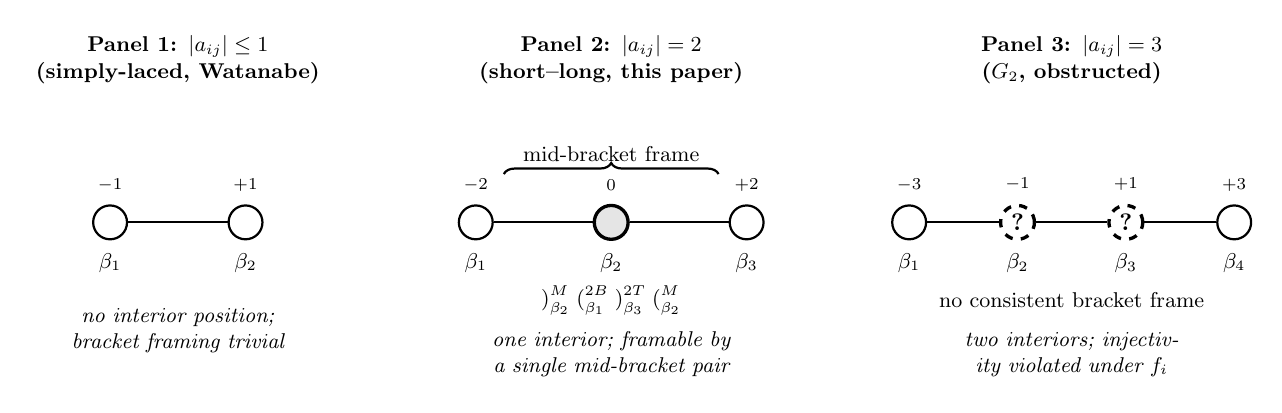
\begin{tikzpicture}[scale=0.86, transform shape,
  every node/.style={font=\small},
  chainnode/.style={circle, draw, thick, minimum size=5mm, inner sep=0pt, fill=white},
  interior/.style={circle, draw, very thick, minimum size=5mm, inner sep=0pt, fill=black!10},
  badinterior/.style={circle, draw, very thick, minimum size=5mm, inner sep=0pt, fill=white, dashed},
  bond/.style={thick},
  brace/.style={decorate, decoration={brace, amplitude=4pt, raise=4pt}, thick},
  panellabel/.style={font=\small\itshape, align=center, text width=4.2cm},
  paneltitle/.style={font=\small\bfseries, align=center}
]

%========== PANEL 1: simply-laced, |a| <= 1 ==========
\begin{scope}[xshift=0cm]
  \node[paneltitle] at (1.0, 2.6) {Panel 1: $|a_{ij}| \leq 1$};
  \node[paneltitle] at (1.0, 2.2) {(simply-laced, Watanabe)};

  \node[chainnode] (a1) at (0, 0) {};
  \node[chainnode] (a2) at (2, 0) {};
  \draw[bond] (a1) -- (a2);

  \node[below=2pt] at (a1.south) {$\beta_1$};
  \node[below=2pt] at (a2.south) {$\beta_2$};
  \node[above=2pt] at (a1.north) {\scriptsize $-1$};
  \node[above=2pt] at (a2.north) {\scriptsize $+1$};

  \node[panellabel] at (1.0, -1.6) {no interior position; bracket framing trivial};
\end{scope}

%========== PANEL 2: short-long, |a| = 2 (this paper) ==========
\begin{scope}[xshift=5.4cm]
  \node[paneltitle] at (2.0, 2.6) {Panel 2: $|a_{ij}| = 2$};
  \node[paneltitle] at (2.0, 2.2) {(short--long, \textbf{this paper})};

  \node[chainnode] (b1) at (0, 0) {};
  \node[interior]  (b2) at (2, 0) {};
  \node[chainnode] (b3) at (4, 0) {};
  \draw[bond] (b1) -- (b2) -- (b3);

  \node[below=2pt] at (b1.south) {$\beta_1$};
  \node[below=2pt] at (b2.south) {$\beta_2$};
  \node[below=2pt] at (b3.south) {$\beta_3$};
  \node[above=2pt] at (b1.north) {\scriptsize $-2$};
  \node[above=2pt] at (b2.north) {\scriptsize $0$};
  \node[above=2pt] at (b3.north) {\scriptsize $+2$};

  \draw[brace] ($(b1.east) + (0.15, 0.55)$) -- ($(b3.west) + (-0.15, 0.55)$)
    node[midway, above=6pt] {mid-bracket frame};

  \node[font=\small, align=center] at (2, -1.15)
    {$\labr{\beta_2}^{M}\;\labl{\beta_1}^{2B}\;\labr{\beta_3}^{2T}\;\labl{\beta_2}^{M}$};

  \node[panellabel] at (2.0, -1.95) {one interior; framable by a single mid-bracket pair};
\end{scope}

%========== PANEL 3: G_2, |a| = 3 ==========
\begin{scope}[xshift=11.8cm]
  \node[paneltitle] at (2.4, 2.6) {Panel 3: $|a_{ij}| = 3$};
  \node[paneltitle] at (2.4, 2.2) {($G_2$, obstructed)};

  \node[chainnode]   (c1) at (0, 0) {};
  \node[badinterior] (c2) at (1.6, 0) {};
  \node[badinterior] (c3) at (3.2, 0) {};
  \node[chainnode]   (c4) at (4.8, 0) {};
  \draw[bond] (c1) -- (c2) -- (c3) -- (c4);

  \node[below=2pt] at (c1.south) {$\beta_1$};
  \node[below=2pt] at (c2.south) {$\beta_2$};
  \node[below=2pt] at (c3.south) {$\beta_3$};
  \node[below=2pt] at (c4.south) {$\beta_4$};
  \node[above=2pt] at (c1.north) {\scriptsize $-3$};
  \node[above=2pt] at (c2.north) {\scriptsize $-1$};
  \node[above=2pt] at (c3.north) {\scriptsize $+1$};
  \node[above=2pt] at (c4.north) {\scriptsize $+3$};

  \node[font=\bfseries] at (c2.center) {?};
  \node[font=\bfseries] at (c3.center) {?};

  \node[font=\small, align=center] at (2.4, -1.15) {no consistent bracket frame};
  \node[panellabel] at (2.4, -1.95) {two interiors; injectivity violated under $f_i$};
\end{scope}

\end{tikzpicture}
\caption{The bracket framework for $\Cmid_a$ admits clean structure only at
$|a_{ij}| \leq 2$: simply-laced edges have no interior (left), the short--long edge has
exactly one interior framable by a single mid-bracket pair (centre, this paper), and the
$G_2$ triple edge has two interiors with no consistent framing (right). Numbers above each
chain node record the pairing $\langle \beta_k, \alpha_i^\vee\rangle$ with the active simple
coroot.}
\label{fig:bracket-trichotomy}
\end{figure}

%==============================================================================
\section{Preliminaries}\label{sec:prelim}
%==============================================================================

\subsection{Notation for type $B_n$}\label{ssec:notation-Bn}

Throughout, $\g$ is the complex simple Lie algebra of type $B_n$ for some $n \geq 2$. We
realise its root system in $\mathbb{R}^n$ with standard basis $E_1, \ldots, E_n$. The simple
roots are
\[
\alpha_a = E_a - E_{a+1} \quad (1 \leq a < n), \qquad \alpha_n = E_n.
\]
The roots $\alpha_1, \ldots, \alpha_{n-1}$ are \emph{long}; $\alpha_n$ is \emph{short}. The
positive roots are
\[
\Phi^+(B_n) \;=\; \{E_a : 1 \leq a \leq n\} \;\cup\; \{E_a - E_b, E_a + E_b : 1 \leq a < b \leq n\}.
\]
The Cartan matrix entries are $a_{a,a+1} = a_{a+1,a} = -1$ for $1 \leq a < n-1$, $a_{n-1,n} =
-2$, $a_{n,n-1} = -1$, and $a_{i,i} = 2$. The entry $a_{n-1,n} = -2$ is the \emph{short--long
edge} that fails $(\mathrm{S1})$--$(\mathrm{S3})'$ of \cite{Watanabe2110}.

We work over a field $\KK$ of characteristic zero throughout (typically $\KK = \mathbb{Q}(q)$
at generic $q$, specialising to $q = 0$ at the crystal limit).

\subsection{Kashiwara crystals and $\imath$-crystals}\label{ssec:kashiwara}

Kashiwara's crystal basis \cite{Kashiwara1991} attaches to each finite-type quantum group
$\Uq$ and each integrable highest-weight module a combinatorial datum $(B, \tilde e_i,
\tilde f_i, \varepsilon_i, \varphi_i, \mathrm{wt})$ obtained as the $q = 0$ limit of a
canonical basis. The lowest-weight crystal $B(\infty)$ of $\Uqm$ admits an explicit realisation
on Kostant partitions:
\[
\Kp(\infty) \;:=\; \bigoplus_{\pi \in \Zn^{\Phi^+}} \KK \cdot \pi,
\]
where each $\pi = (c_\beta)_{\beta \in \Phi^+}$ is a vector of nonnegative root multiplicities
and the Kashiwara operators $\tilde e_i, \tilde f_i$ are computed by the bracketing procedure
recalled in Section~\ref{ssec:bracket-alphabet}.

\medskip
\noindent\textbf{The $\imath$-crystal extension.}
For a quantum symmetric pair $(\Uq, \Uiota)$ of finite type, the $\imath$-coideal subalgebra
$\Uiota$ is generated by symbols $B_i = F_i + \varsigma_n T_i(\Theta)$ that twist the Chevalley
$F_i$ by Kashiwara--Lusztig-style adjoint terms. At $q = 0$, $B_i$ specialises to a
single combinatorial operator on $\Kp(\infty)$ which Watanabe \cite{Watanabe2107} writes as
\[
B_i \;=\; \tilde e_i + \tilde f_i \quad (\text{at } q = 0)
\]
when the node $i$ is split, i.e., $a_{i,\tau(i)} = 2$. (Other cases of $a_{i,\tau(i)} \in
\{0, -1\}$ give different combinatorial operators; see \cite[\S4.1]{Watanabe2110}.) The pair
$(\Kp(\infty), B_i)$ for $i$ ranging over the Satake diagram is the \emph{$\imath$-crystal}
of $\Uiota$ at the chosen quantum symmetric pair.

For type BDI, $\tau = \mathrm{id}$, so every node is split and $a_{i,\tau(i)} = 2$ for all $i$.
The combinatorial operator $B_i = \tilde e_i + \tilde f_i$ acts on $\Kp(\infty)$ for each
simple root $\alpha_i$. The present paper studies the case $i = n$, the short simple.

\begin{remark}[Parameter convention for $\varsigma_n$]\label{rmk:varsigma-convention}
Following Watanabe \cite[\S3.3(D)]{Watanabe2110}, the parameter $\varsigma_n$ lies in
$\{q_n^a : a \in \mathbb{Z}\}$; the main theorem is independent of the choice of
$\varsigma_n$ in this set, so we normalise $\varsigma_n = 1$ in computations.
\end{remark}

\subsection{The bracket alphabet}\label{ssec:bracket-alphabet}

The Kashiwara operators are computed via a bracket-sequence procedure that we now recall in
the form used throughout the paper. This is the CST formulation of \cite[Definition~2.14]{CST}
(see also Salisbury--Tingley); we extend the standard signature to handle the doubled
contribution at $a_{ij} = -2$.

\medskip
\noindent\textbf{Symbols.}
The bracket alphabet consists of two symbols, $\labl{}$ (raising) and $\labr{}$ (lowering),
each carrying a label in $\Phi^+$. Concatenations of bracket symbols form bracket sequences.
The number of symbols an individual root $\beta$ contributes is governed by its pairing with
the simple coroot $\alpha_i^\vee$ at which we read brackets:
\[
\#\text{ of }\labr{\beta}\text{s contributed per multiplicity of }\beta \;=\; \max(0,\;\langle
\beta, \alpha_i^\vee\rangle), \qquad
\#\text{ of }\labl{\beta}\text{s} \;=\; \max(0,\;-\langle \beta, \alpha_i^\vee\rangle).
\]
For the short simple of $B_n$, the pairings are $\langle E_a - E_n, \alpha_n^\vee\rangle =
-2$, $\langle E_a, \alpha_n^\vee\rangle = 0$, $\langle E_a + E_n, \alpha_n^\vee\rangle = +2$,
and $\langle E_n, \alpha_n^\vee\rangle = +2$. The middle case requires care: the root $E_a$
with $\langle E_a, \alpha_n^\vee\rangle = 0$ contributes both raising and lowering symbols
because it has nonzero $\alpha_n$-string length, namely both $E_a + E_n$ and $E_a - E_n$ are
in $\Phi^+$. The standard convention (see \cite[\S2]{Kashiwara1991}) places one $\labr{E_a}$
per multiplicity \emph{before} the contributions of $E_a + E_n, E_a - E_n$ and one
$\labl{E_a}$ \emph{after}.

\medskip
\noindent\textbf{Cancellation.}
The bracket sequence is canonicalised by repeated cancellation: any adjacent pair $\labl{}
\labr{}$ (a raising symbol immediately followed by a lowering symbol) is removed. The
process terminates and produces a canonical sequence with all surviving $\labr{}$s to the
left of all surviving $\labl{}$s. The cancellation respects bracket labels in the sense that
the labels do not affect which symbols cancel, only what label appears on the resulting
operator.

\medskip
\noindent\textbf{Operators from brackets.}
Given the canonical bracket sequence of $\pi$ at the simple root $\alpha_i$:
\begin{itemize}[leftmargin=2em]
  \item $\varepsilon_i(\pi)$ is the number of surviving $\labr{}$s.
  \item $\varphi_i(\pi)$ is the number of surviving $\labl{}$s.
  \item $\tilde e_i(\pi)$ acts on the rightmost surviving $\labr{}$, with label $\beta$; the
    action on $\pi$ is $\pi \mapsto \pi - e_\beta + e_{\beta - \alpha_i}$ when $\beta \neq
    \alpha_i$, and $\pi \mapsto \pi - e_{\alpha_i}$ when $\beta = \alpha_i$.
  \item $\tilde f_i(\pi)$ acts on the leftmost surviving $\labl{}$ symmetrically.
\end{itemize}

\medskip
\noindent\textbf{Extension at $a_{ij} = -2$.}
The convention above gives the doubled exponents naturally: the root $E_a + E_n$, having
$\langle \cdot, \alpha_n^\vee\rangle = 2$, contributes $\labr{E_a + E_n}^2$ per multiplicity,
and similarly $E_a - E_n$ contributes $\labl{E_a - E_n}^2$ per multiplicity. These doubled
symbol counts are the bracket-level expression of the short--long Cartan entry $|a_{n,a}|
= 2$.

\subsection{The slice $K_p(\infty)$ and step types}\label{ssec:slice}

For the rest of the paper we fix the short simple $i = n$ and abbreviate $\varepsilon =
\varepsilon_n$, $\varphi = \varphi_n$, $\tilde e = \tilde e_n$, $\tilde f = \tilde f_n$, and
write $B := B_n = \tilde e + \tilde f$ for the $\imath$-coideal generator at the short node.

\begin{definition}\label{def:slice}
The \emph{depth-$k$ slice} of $\Kp(\infty)$ at the short simple is
\[
S_n^{(k)} \;:=\; \{\pi \in \Kp(\infty) : \varepsilon(\pi) \geq k\}.
\]
For $k = 2$ we abbreviate $S_n := S_n^{(2)}$ and call it simply the \emph{slice} (or
\emph{on-slice} part) when the value of $k$ is clear from context.
\end{definition}

The combinatorial object of central interest is the multiset of net deltas of $\tilde e^2$
on the slice:
\[
C_n \;:=\; \bigl\{\,\tilde e^2(\pi) - \pi \;:\; \pi \in S_n\,\bigr\},
\]
called the \emph{$e_n^2$ catalog}. The size of this catalog and its structural decomposition
into three classes are the empirical content that the tensor product rule will explain.

\medskip
\noindent\textbf{$\alpha_n$-orbits on $\Phi^+$.}
The action of the short reflection $s_n$ partitions $\Phi^+(B_n)$ into three families:

\begin{itemize}[leftmargin=2em]
  \item \emph{Chains.} For each $a \in \{1, \ldots, n-1\}$,
    \[
    \Chain(a) \;=\; \{E_a - E_n,\; E_a,\; E_a + E_n\}
    \]
    is a length-three $\alpha_n$-string with $E_a$ as the middle root.
  \item \emph{Singleton.} $\Sing = \{E_n\}$, a length-one $\alpha_n$-string. ($\alpha_n$
    itself.)
  \item \emph{Non-touching.} $\NT = \{E_a \pm E_b : 1 \leq a < b < n\}$, length-one
    $\alpha_n$-strings with $\langle \cdot, \alpha_n^\vee\rangle = 0$ and with no neighbouring
    root in $\Phi^+ \cup \{0\}$ across $\pm \alpha_n$.
\end{itemize}

The non-touching roots contribute no bracket symbols at $\alpha_n$ (raising and lowering
counts both zero) and so play no role in the $B_n$-action. We omit them from the tensor
product decomposition; see Remark~\ref{rmk:non-touching-phaseB} for the bookkeeping needed
if one wishes to include them as trivial factors.

\subsection{Step types}\label{ssec:step-types}

\begin{definition}\label{def:step-types}
The \emph{step types} of $\tilde e$ on $\Kp(\infty)|_{B_n}$ are the labelled actions on
$\pi$ that arise from acting on a rightmost surviving $\labr{}$ at the short simple. They are:
\begin{align*}
\MB(a) &: \quad \pi \mapsto \pi - e_{E_a} + e_{E_a - E_n}, \quad a \in \{1, \ldots, n-1\}, \\
\TM(a) &: \quad \pi \mapsto \pi - e_{E_a + E_n} + e_{E_a}, \quad a \in \{1, \ldots, n-1\}, \\
\Sing &: \quad \pi \mapsto \pi - e_{E_n}.
\end{align*}
\end{definition}

The labels MB and TM are mnemonics: MB ``mid drops to bot'' and TM ``top drops to mid'' along
the chain. There are $2(n-1) + 1 = 2n - 1$ step types in total.

\subsection{The chain factor and singleton factor}\label{ssec:factors}

We now define the two building blocks of the tensor product decomposition.

\begin{definition}[Chain factor]\label{def:chain-factor}
For each $a \in \{1, \ldots, n-1\}$, the \emph{chain factor} is the $\Zn^3$-graded vector space
\[
\Cmid_a \;:=\; \KK\bigl\langle (M, B, T) : M, B, T \in \Zn \bigr\rangle
\]
on three generators of grades $E_a$ (\emph{mid}), $E_a - E_n$ (\emph{bot}), $E_a + E_n$
(\emph{top}). Its \emph{internal bracket block} at the short simple $\alpha_n$ is the bracket
sequence
\begin{equation}\label{eq:chain-bracket-block}
\br(\Cmid_a)(M, B, T) \;=\; \labr{E_a}^{M}\;\labl{E_a - E_n}^{2B}\;\labr{E_a + E_n}^{2T}\;\labl{E_a}^{M}.
\end{equation}
\end{definition}

\begin{definition}[Singleton factor]\label{def:singleton-factor}
The \emph{singleton factor} is the $\Zn$-graded vector space
\[
\Csing \;:=\; \KK[B_n] \;\cong\; \bigoplus_{S \geq 0} \KK \cdot B_n^S,
\]
i.e., the polynomial algebra on the generator $B_n$ itself. Its internal bracket block at
the short simple is
\begin{equation}\label{eq:sing-bracket-block}
\br(\Csing)(S) \;=\; \labr{E_n}^{S}.
\end{equation}
\end{definition}

\begin{remark}[Doubling and the short--long edge]\label{rmk:doubling}
The doubled exponents $2B$ and $2T$ in (\ref{eq:chain-bracket-block}) are the bracket-level
realisation of the off-diagonal Cartan entries
\[
\langle E_a - E_n, \alpha_n^\vee\rangle \;=\; -2, \qquad \langle E_a + E_n, \alpha_n^\vee\rangle \;=\; +2,
\]
equivalent to $|a_{n,a}| = 2$ for the short--long edge. The mid-framing $\labr{E_a}^M \cdots
\labl{E_a}^M$ is the bracket-level expression of $\langle E_a, \alpha_n^\vee\rangle = 0$
combined with the fact that $E_a$ has a non-trivial $\alpha_n$-string of length three; the
mid root contributes both raising and lowering symbols, with the bot- and top-contributions
sandwiched between them.
\end{remark}

\begin{remark}[Comparison with Watanabe]\label{rmk:watanabe-vs-chain}
The singleton factor $\Csing$ is exactly Watanabe's split-node rank-one $\imath$-crystal
$U^n_n = \KK[B_n]$ from \cite[\S4.1]{Watanabe2110} at the split node $a_{n,\tau(n)} = 2$.
The chain factor $\Cmid_a$ has no counterpart in \cite{Watanabe2110}: the framework there has
only rank-one per-node objects glued by simply-laced edges, and the short--long edge $a_{n-1,n}
= -2$ requires the new rank-three building block $\Cmid_a$ to encode the doubled bracket
contribution.
\end{remark}

\begin{notation}[Chain--sing coordinates]\label{not:chain-sing}
Throughout the rest of the paper we record a Kostant partition $\pi \in \Kp(\infty)$ by its
\emph{chain--sing coordinates}
\[
   \bigl((M_a, B_a, T_a)_{a = 1}^{n - 1},\;\; S,\;\; \piNT\bigr),
\]
where $(M_a, B_a, T_a) \in \Zn^3$ is the multidegree of $\pi$ in the chain factor $\Cmid_a$
($M_a, B_a, T_a$ count the multiplicities of $E_a, E_a - E_n, E_a + E_n$ respectively),
$S \in \Zn$ is the multidegree of $\pi$ in the singleton factor $\Csing$ (the multiplicity
of $E_n$), and
\[
   \piNT \;\in\; \Zn^{\NT}
\]
collects the non-touching multiplicities $(c_\beta)_{\beta \in \NT}$ of $\pi$ on $\NT =
\{E_a \pm E_b : 1 \le a < b < n\}$. The components $\piNT$ contribute no bracket symbols at
$\alpha_n$ and are fixed under the $B_n$-action (Remark~\ref{rmk:non-touching-phaseB}); they
enter the analytical content of \S\ref{sec:carry} only through their disjoint sublattice.

Section~\ref{sec:carry} introduces, on the chain--sing coordinates, the cumulative carry
$P_a := \sum_{b \le a} 2(B_b - T_b)$ (Definition~\ref{def:carry}), the chain highest-weight
polytope $\Pn_n$ (Definition~\ref{def:chain-polytope}), the chain-to-weight map $\Phi$
($\S\ref{ssec:weight-simplicial}$), and the descent recording set $\Rec(\pi^{\hw})$
($\S\ref{ssec:carry-descent}$).
\end{notation}

%==============================================================================
% v3 §3: The cumulative carry P_a as analytical backbone.
% (Replaces v2's §3 "Main theorem and Phase A".)
%==============================================================================
% ==============================================================================
% v3 BDI §3 — The cumulative carry $P_a$ as analytical backbone
% Standalone fragment; to be \input{} into v3 main.tex.
% ==============================================================================
%
% Macros the v3 preamble must provide (inherited from v2 main.tex unless flagged NEW):
%
%   \Kp, \NT, \Sing, \Chain, \MB, \TM, \Cmid, \Csing, \KK, \Z, \Zn,
%   \g, \eps, \labr, \labl                                            (v2)
%
%   \newcommand{\Pcum}{P^{\mathrm{cum}}}                              (NEW)
%   \newcommand{\Pn}{\mathcal{P}}                                     (NEW; chain polytope)
%   \newcommand{\hw}{\mathrm{hw}}                                     (NEW)
%   \newcommand{\piNT}{\pi^{\NT}}                                     (NEW)
%   \newcommand{\Rec}{\mathcal{R}}                                    (NEW; recording set)
%   \newcommand{\HW}{\mathrm{HW}}                                     (NEW)
%   \DeclareMathOperator{\wt}{wt}                                     (NEW)
%
% Theorem environments are those declared in v2: theorem, proposition, lemma,
% corollary, definition, example, remark.  Numbering continues from \section{}.
% ==============================================================================

\section{The cumulative carry $P_a$ as analytical backbone}\label{sec:carry}

%-------------------------------------------------------------------------------
\subsection{Roadmap}\label{ssec:carry-roadmap}

Throughout this section $\g$ is of type $B_n$, $n \ge 2$, and $\pi \in \Kp(\infty)$
has the chain--sing coordinates
\[
   \bigl((M_a, B_a, T_a)_{a=1}^{n-1},\; S,\; \piNT\bigr)
\]
of \S\ref{sec:prelim}. We isolate a single scalar, the \emph{cumulative carry}
\[
   P_a \;:=\; \sum_{b=1}^{a} 2(B_b - T_b), \qquad P_0 := 0,
\]
and show that it carries the entire short-simple analytic content of the
chain--singleton decomposition at $B_n$. The carry plays five structurally
distinct roles, the first four forced by the single left-to-right bracket scan
of Theorem~\ref{thm:carry-A}, the fifth obtained from the first by Farkas-polar:

\begin{enumerate}[label=(R\arabic*),leftmargin=2.5em]
  \item \textbf{Descent recording} (\S\ref{ssec:carry-descent}). $P_a$ is one-sided
    monotone along forward $\widetilde{e}_n$-descent. This obstructs any local
    witness for the image $\Rec(\pi^{\hw})$, closing v3 OPEN-3 by impossibility.
  \item \textbf{Singleton cross-chain coupling} (\S\ref{ssec:carry-cross}). The
    unique cross-chain condition in the $B_n$-highest indicator is the carry
    sum lift $[\,S \le P_{n-1}\,]$, type-uniform in $n$.
  \item \textbf{Carry-recursive factorisation} (\S\ref{ssec:carry-factor}). Per-chain
    MB and TM tests couple chain $a$ to all prior chains through $P_{a-1}$;
    the $B_n$-HW indicator factors carry-recursively, not as a strict tensor.
  \item \textbf{Polytope completeness} (\S\ref{ssec:carry-polytope}). The chain-side
    HW polytope $\Pn_n$ has exactly $2n - 3$ non-redundant carry-derived facets,
    namely $\{L_a, U_a : 2 \le a \le n-1\} \cup \{E\}$, with $L_1$ degenerate
    and $U_1$ redundant.
  \item \textbf{Weight-space simplicial cone} (\S\ref{ssec:weight-simplicial}).
    Under the chain-to-weight map $\Phi$, the image cone $\Kp_n \subset
    \mathbb{R}^n$ is simplicial with exactly $n$ facets; of the $2n - 3$
    chain-side carry-derived facets, only $E$ survives projection, and the
    chain-to-weight contraction has ratio $(2n - 3)/n \to 2$.
\end{enumerate}

External polyhedral and algebraic shadows are recorded in
\S\ref{ssec:kobayashi-fences} (Kobayashi) and \S\ref{ssec:carry-shadows}
(Watanabe, Meereboer, Frohmader); the closing remark (\S\ref{ssec:carry-closing})
collects the five roles as five views of one object.

%-------------------------------------------------------------------------------
\subsection{The cumulative carry $P_a$ and Theorem A}\label{ssec:carry-Pa}

We recall the chain--sing alphabet of \S\ref{sec:prelim}. For each
$a = 1, \dots, n-1$, the chain-$a$ multiplicities $(M_a, B_a, T_a)$ count the
roots $(E_a,\, E_a - E_n,\, E_a + E_n)$ respectively; the singleton multiplicity
$S$ counts $E_n$. The non-touching block $\piNT$ contributes no bracket symbols
at $\alpha_n$ and is fixed under the $B_n$-action; it plays no role in this
section, and we drop it from notation after Lemma~\ref{lem:carry-mono}.

The CST bracket sequence $S_n(\pi)$ for the short simple $\alpha_n$ is the
left-to-right concatenation, for $a = 1, \dots, n-1$, of the per-chain block
\[
   \labr{E_a}^{M_a}\;\labl{E_a - E_n}^{2 B_a}\;\labr{E_a + E_n}^{2 T_a}\;\labl{E_a}^{M_a},
\]
followed by the singleton block $\labr{E_n}^{S}$. Standard cancellation defines
$\eps_n(\pi)$.

\begin{definition}[Cumulative carry]\label{def:carry}
Set $P_0 := 0$ and, for $a = 1, \dots, n-1$,
\[
   P_a \;:=\; P_{a-1} + 2(B_a - T_a) \;=\; \sum_{b=1}^{a} 2(B_b - T_b).
\]
We occasionally write $\Pcum_a$ when the cumulative nature is the focus.
\end{definition}

Up to sign, $P_a = -\langle \alpha_n^\vee,\, \wt(\pi)|_{\le a}\rangle$: the carry
records twice the cumulative deficit of $E_n$-content over chains $1, \dots, a$.

\begin{lemma}[One-sided monotonicity]\label{lem:carry-mono}
Each forward chain-factor descent step ($\widetilde{e}_n$ acting on the rightmost
surviving $\labr{}$ in $S_n(\pi)$) adjusts $P_a$ as follows:
\begin{itemize}[leftmargin=2em]
  \item $\Sing$: $S \mapsto S - 1$; no change to any $P_a$.
  \item $\MB(a)$: $(M_a, B_a, T_a) \mapsto (M_a - 1, B_a + 1, T_a)$; $P_b \mapsto P_b + 2$ for $b \ge a$.
  \item $\TM(a)$: $(M_a, B_a, T_a) \mapsto (M_a + 1, B_a, T_a - 1)$; $P_b \mapsto P_b + 2$ for $b \ge a$.
\end{itemize}
No letter decreases any $P_a$ under forward descent.
\end{lemma}

\begin{proof}
Direct from Definitions~\ref{def:step-types} and~\ref{def:carry}.
\end{proof}

The next statement is Theorem~A in carry form, with $P_a$ as the load-bearing
object. It is the master lemma on which \S\ref{ssec:carry-descent}--\S\ref{ssec:weight-simplicial} rest.

\begin{theorem}[Theorem~A in carry form]\label{thm:carry-A}
$\eps_n(\pi) = 0$ if and only if
\begin{align}
   (\HW_a) \quad & M_a \le P_{a-1} \;\text{ and }\; M_a \le P_a,
   && a = 1, \dots, n-1, \label{eq:carry-HWa}\\
   (\HW_{\mathrm{sing}}) \quad & S \le P_{n-1}. \label{eq:carry-HWsing}
\end{align}
\end{theorem}

\begin{proof}
A left-to-right scan of $S_n(\pi)$ tracking the running open-paren count $Q$. By
induction on $a$, on entry to chain $a$ we have $Q = P_{a-1}$ provided no
$\labr{}$ has survived; the chain-$a$ subscan survives a $\labr{}$ in exactly
the cases excluded by~\eqref{eq:carry-HWa}, after rewriting the second of the
two original inequalities ($M_a + 2 T_a \le P_{a-1} + 2 B_a$) as $M_a \le P_a$.
The singleton block then processes against $Q = P_{n-1}$, giving
\eqref{eq:carry-HWsing}.
\end{proof}

We use the clean form~\eqref{eq:carry-HWa} throughout the remainder of the section.

%-------------------------------------------------------------------------------
\subsection{Descent role: no local witness}\label{ssec:carry-descent}

Theorem~B (\S\ref{sec:phaseB}) makes the descent step
$\pi \mapsto (\pi^{\hw}, R(\pi))$ a bijection
\[
   \Kp(\infty)/B_n \;\longrightarrow\; \bigsqcup_{\pi^{\hw}} \{\pi^{\hw}\} \times \Rec(\pi^{\hw}),
\]
where $\Rec(\pi^{\hw})$ is the set of valid recording words. The natural question
(v3 OPEN-3) is whether $\Rec(\pi^{\hw})$ admits a \emph{local} characterisation:
a finite list of prefix/suffix inequalities on a candidate word $R$ that
decides membership without replaying the descent.

\begin{proposition}[No local witness]\label{prop:no-local-witness}
There is no signed prefix or suffix invariant on the recording word $R$ whose
non-negativity (or vanishing) characterises $R \in \Rec(\pi^{\hw})$.
\end{proposition}

\begin{proof}
By Lemma~\ref{lem:carry-mono}, every forward step adds $0$ or $+2$ to each $P_b$
and never decreases any. The reverse-played word therefore monotonically
\emph{drains} $P_b$. For a candidate word $R$ that is not in $\Rec(\pi^{\hw})$,
intermediate states during reverse-play can drive some $P_b$ arbitrarily
negative with no later letter able to compensate; the failure cannot be diagnosed
by any signed counter on $R$ alone. The only correct test is the oracle: $R \in
\Rec(\pi^{\hw})$ iff reverse-playing $R$ from $\pi^{\hw}$ stays coordinate-nonnegative
and forward descent of the resulting Kostant partition recovers $R$.
\end{proof}

Proposition~\ref{prop:no-local-witness} is supported by a three-probe falsification
arc on the candidate inequalities (i)~prefix carry $\ge 0$, (i$'$)~pair-aware
prefix carry, (iii)~per-chain suffix balance. All three give zero false positives
and monotonically growing false negatives ($268, 360, 410$) as the candidate
tightens: the signature of an impossibility, not a tuning miss.

\begin{remark}[Asymmetric mirror]\label{rmk:asymmetric-mirror}
Lemma~\ref{lem:carry-mono} is the analytical heart of an
\emph{asymmetric-mirror} phenomenon: forward and
reverse descent are not exchanged by a local involution because the alphabet
$\{\Sing, \MB(a), \TM(a)\}$ has no signed compensator at the carry level. The
chain-factor alphabet is rank-3, but the carry sees only a $\{0, +2\}$ bit. The
signed slack data $(t_0^{(i)}, r^{(i)})$ that Azenhas's type-AII recording
exploits has no chain-factor analogue: $\MB(a)$ and $\TM(a)$ are distinct
chain-factor bits but contribute identically to $P_a$. This is the
rank-3-chain-factor-vs-rank-1-strip distinction of \S\ref{ssec:scope} at the
analytic level, and it is why no local witness exists for $\Rec(\pi^{\hw})$.
\end{remark}

%-------------------------------------------------------------------------------
\subsection{Projection role: Theorem E}\label{ssec:carry-cross}

The second role of the carry is to mediate the unique cross-chain condition in
the $B_n$-highest indicator.

\begin{theorem}[Singleton cross-chain coupling]\label{thm:carry-E}
Let $\pi \in \Kp(\infty)$ have chain--sing coordinates
$((M_a, B_a, T_a)_{a=1}^{n-1}, S)$. Then $\pi$ is $B_n$-highest if and only if
\[
   (\HW_a) \quad M_a \le P_{a-1}\ \text{and}\ M_a \le P_a, \quad a = 1, \dots, n-1,
\]
\[
   (\HW_{\mathrm{sing}}) \quad S \le P_{n-1} \;=\; \sum_{a=1}^{n-1} 2(B_a - T_a).
\]
In particular, the only cross-chain condition is the cumulative carry bound
\[
   \mathrm{Cross}(M, B, T, S) \;=\; [\,S \le P_{n-1}\,] \;=\; \Bigl[\, S \le \sum_{a=1}^{n-1} 2(B_a - T_a) \,\Bigr],
\]
which depends only on the final cumulative carry and is type-uniform in $n$.
\end{theorem}

\begin{proof}
The biconditional is Theorem~\ref{thm:carry-A}. The proof there is a single
left-to-right scan whose recurrence and per-block surviving-bracket count have
no $n$-dependence beyond the chain index, and whose singleton block always
processes against $P_{n-1}$.
\end{proof}

\begin{remark}[The NT block contributes zero]\label{rmk:NT-drop}
The non-touching block $\piNT$ contributes no bracket symbols at $\alpha_n$
(every non-touching root has $\langle \cdot, \alpha_n^\vee\rangle = 0$ and trivial
$\alpha_n$-string), so it appears in neither $S_n(\pi)$ nor any $P_a$. The cross-chain
sum~\eqref{eq:carry-HWsing} therefore reads against the chain--sing coordinates
alone, and $\piNT$ is free under the $B_n$-action. This is the silent assumption
underlying Theorem~\ref{thm:carry-E} and Corollary~\ref{cor:carry-factor}: every analytic
identity at $\alpha_n$ is invariant under arbitrary changes to $\piNT$.
\end{remark}

\begin{example}[Singleton draws on cumulative carry]\label{ex:carry-cross-B4}
At $B_4$ the configuration $(M, B, T, S) = ((0,0,0), (0,1,0), (0,0,0),\, 2)$ has
$P_1 = 0$, $P_2 = 2$, $P_3 = 2$, so $S = 2 = P_{n-1}$ and the configuration is
$B_4$-highest with all $(\HW_a)$ trivially satisfied. The singleton capacity
is supplied by chain~$2$ alone, confirming that the cross-chain condition is
genuinely cumulative, not pointwise per-chain.
\end{example}

Empirically, on the $1716$ chain+sing configurations at $B_3$, content $\le 6$,
the sum-lift $[S \le P_{n-1}]$ is the unique candidate (among pointwise
$\bigwedge_a [S \le 2(B_a - T_a)]$, sum lift, cumulative-and, min, max) with zero
false negatives; the same dataset falsifies the strict tensor factorisation
``$\chi_1(M_1, B_1, T_1) \cdot \chi_2(M_2, B_2, T_2) \cdot \mathrm{Cross}$'' with
$34$ inconsistent $(\mathrm{chain}_1, \Delta P_2, S)$-keys. A $B_4$ spot check
($3003$ configurations at content $\le 5$) gives $3003/3003$. Full write-up:
\url{proofs/2026-05-20-pnu-Bn-cross-chain.md}.

%-------------------------------------------------------------------------------
\subsection{Carry-recursive factorisation}\label{ssec:carry-factor}

Theorem~\ref{thm:carry-E} admits an immediate corollary in factorised form.

\begin{corollary}[Carry-recursive factorisation]\label{cor:carry-factor}
The $B_n$-HW indicator factors as
\[
   [\,B_n\text{-HW}(M, B, T, S)\,]
   \;=\; \prod_{a=1}^{n-1} \chi_a(M_a, B_a, T_a;\, P_{a-1}) \,\cdot\, [\,S \le P_{n-1}\,],
\]
with $\chi_a = [M_a \le P_{a-1}] \wedge [M_a \le P_a]$ and the carry update
$P_a = P_{a-1} + 2(B_a - T_a)$, $P_0 = 0$.
\end{corollary}

The factorisation is \emph{carry-recursive}, not strict tensor: $\chi_a$ depends
on the incoming scalar $P_{a-1}$ as well as on $(M_a, B_a, T_a)$, and the
singleton factor uses $P_{n-1}$. As in Remark~\ref{rmk:NT-drop}, the NT block
contributes neither to the per-chain factors $\chi_a$ nor to the singleton
bound, so it is absent from the corollary. Corollary~\ref{cor:carry-factor} is
the unified replacement for the descent-recording and projection-cross-chain
results of the old v3 outline: both follow from a single left-to-right bracket
scan acting on a single scalar.

%-------------------------------------------------------------------------------
\subsection{Polytope completeness (Theorem~F)}\label{ssec:carry-polytope}

The fourth role of the carry is structural. The system $(\HW_a) \cup
(\HW_{\mathrm{sing}})$ of Theorem~\ref{thm:carry-A} is a list of $2n - 1$ linear
inequalities; we ask how many of them are non-redundant facets of the
chain-side HW polytope, and which.

\begin{definition}[Chain HW polytope]\label{def:chain-polytope}
The \emph{chain HW polytope} at $B_n$ is
\[
   \Pn_n \;:=\; \bigl\{ (M, B, T, S) \in \Z_{\ge 0}^{3(n-1) + 1} : \pi \text{ is } B_n\text{-highest} \bigr\}
\]
(viewing $\Pn_n$ as a lattice polytope, equivalently the intersection of
non-negativity with the carry system).
\end{definition}

Label the $2n - 1$ carry-derived inequalities of $\Pn_n$ as
\[
   L_a : M_a \le P_{a-1}, \quad U_a : M_a \le P_a \qquad (1 \le a \le n - 1),
   \qquad E : S \le P_{n-1}.
\]

\begin{theorem}[Polytope completeness]\label{thm:carry-F}
Let $n \ge 2$. The chain HW polytope $\Pn_n$ has exactly $2n - 3$ non-redundant
carry-derived facets, namely
\[
   \{L_a, U_a : 2 \le a \le n-1\} \;\cup\; \{E\}.
\]
The boundary inequalities at $a = 1$ are special:
\begin{enumerate}[label=(\roman*),leftmargin=2em]
  \item $L_1$ is \emph{degenerate}: it is non-redundant as an inequality but is
    saturated on every $\pi \in \Pn_n$, forcing $M_1 = 0$ identically. Equivalently,
    $\Pn_n$ lies in the affine hyperplane $\{M_1 = 0\}$.
  \item $U_1$ is \emph{redundant}: it is implied by $L_1$ together with non-negativity
    of $M_2$ (for $n \ge 3$) or of $S$ (for $n = 2$), via $L_2 + (M_2 \ge 0)$
    respectively $E + (S \ge 0)$.
\end{enumerate}
\end{theorem}

\begin{proof}
\emph{(i)~$L_1$ degenerate.} $L_1$ reads $M_1 \le P_0 = 0$. With $M_1 \ge 0$,
this forces $M_1 = 0$ on $\Pn_n$. Non-redundancy: the configuration
$(M_1, B_1, T_1) = (1, 1, 0)$ (other coordinates zero) has $P_1 = 2$ and
satisfies every $L_a, U_a$ for $a \ge 2$ and $E$ (each reads against $M_a = 0$
or $S = 0$ with $P_{n-1} = 2$), but violates $L_1$. So $L_1$ is needed; on
$\Pn_n$ it is always tight.

\emph{(ii)~$U_1$ redundant.} By (i), $M_1 = 0$ on $\Pn_n$, so $U_1$ becomes the
slack inequality $0 \le P_1$. If $n = 2$, fence $E$ reads $S \le P_1$ and
non-negativity gives $P_1 \ge S \ge 0$. If $n \ge 3$, fence $L_2$ reads
$M_2 \le P_1$ and non-negativity gives $P_1 \ge M_2 \ge 0$. Either way, the
other inequalities together with non-negativity force $U_1$.

\emph{(iii)~$\{L_a, U_a : 2 \le a \le n-1\} \cup \{E\}$ are non-redundant.} For
each, we exhibit a chain configuration that satisfies every \emph{other}
inequality of the system but violates the named one (existence of such a witness
proves non-redundancy; saturation then has a relative-interior point, giving a
codimension-$1$ face).

\smallskip
\noindent\textit{Witness for $L_a$ ($2 \le a \le n-1$):} set $M_a = 1$,
$B_a = 1$, all other coordinates zero. Then $P_b = 0$ for $b < a$ and $P_b = 2$
for $b \ge a$. Every $L_b, U_b$ for $b < a$ has $M_b = 0 \le 0$; $U_a$ reads
$1 \le 2$; every $L_b, U_b$ for $b > a$ reads $0 \le 2$; $E$ reads $0 \le 2$;
$L_a$ reads $1 \le 0$ and is the unique violation.

\smallskip
\noindent\textit{Witness for $U_a$ ($2 \le a \le n-1$):} set $M_a = 1$,
$B_{a-1} = 1$, $T_a = 1$, all other coordinates zero. Then $P_b = 0$ for
$b < a-1$, $P_{a-1} = 2$, $P_b = 0$ for $b \ge a$. $L_a$ reads $1 \le 2$;
$U_a$ reads $1 \le 0$ and is the unique violation; all others are slack.

\smallskip
\noindent\textit{Witness for $E$:} set $S = 1$, all chain coordinates zero. Then
$P_{n-1} = 0$; every $L_a, U_a$ reads $0 \le 0$; $E$ reads $1 \le 0$ and is the
unique violation.

\smallskip
\noindent To upgrade non-redundancy to codimension-$1$, type-uniform
relative-interior witnesses are constructed in
\texttt{verify\_facet\_interiors.py} (verified at $n = 3, \dots, 7$); we sketch:
for $L_a$, take $B_b = 1$ ($1 \le b \le a-1$), $M_a = 2(a-1)$, $B_a = 1$, giving
$L_a$ saturated and all others strict; for $U_a$ ($a \ge 3$), take the same
prefix with $M_a = 2(a-2)$, $T_a = 1$, $B_a = 0$, giving $U_a$ saturated and all
others strict; for $U_2$, take $B_1 = 2$, $M_2 = 2$, $T_2 = 1$; for $E$, take
$B_b = 1$ ($1 \le b \le n-1$), $S = 2(n-1)$.
\end{proof}

\begin{remark}[Boundary behaviour]\label{rmk:boundary-asymmetry}
The asymmetry at $a = 1$ is structural rather than incidental: the carry
recursion starts at $P_0 = 0$, so $L_1$ is the strongest possible mid-bound
($M_1 \le 0$) and $U_1$ is the corresponding slack form ($P_1 \ge 0$) that the
next downstream constraint enforces. Internally ($2 \le a \le n-1$), $P_{a-1}$
and $P_a$ both range over positive values and neither is universally tighter,
so both $L_a$ and $U_a$ contribute honest facets.
\end{remark}

\begin{remark}[Computational verification]\label{rmk:carry-F-verification}
The script \texttt{verify\_witnesses.py} verifies the three-class structure
($L_1$ degenerate, $U_1$ redundant, all other carry-derived inequalities
non-redundant) for $n \le 7$, and \texttt{classify\_fences.py} enumerates all
chain configurations of total content $\le C$ at $B_n$, $n \le 6$, classifying
each inequality by saturation count, strict-satisfaction count, and explicit
non-redundancy count. The polytope-completeness data table (Day-$28$ proof,
\url{proofs/2026-05-21-bdi-kobayashi-faces.md}) records the explicit
non-redundancy counts at $(n, C) = (2, 8), (3, 6), (4, 6), (5, 4), (6, 3)$.
\end{remark}

The polytope role completes the chain-side unification: $P_a$ is the analytical
backbone in \S\ref{ssec:carry-Pa}, the descent potential in
\S\ref{ssec:carry-descent}, the cross-chain coupling in
\S\ref{ssec:carry-cross}, the recursive scalar in \S\ref{ssec:carry-factor},
and the facet-counting object in \S\ref{ssec:carry-polytope}. The same scan
that proves Theorem~\ref{thm:carry-A} proves all four. The fifth role
(\S\ref{ssec:weight-simplicial}) is obtained from the same chain-side data by
Farkas-polar under the chain-to-weight projection $\Phi$.

%-------------------------------------------------------------------------------
\subsubsection{Weight-space image is simplicial (Theorem~G)}\label{ssec:weight-simplicial}

Theorem~\ref{thm:carry-F} counts the carry-derived facets of $\Pn_n$ on the
chain side, in the $3(n-1) + 1$ chain--singleton coordinates. The
representation-theoretic object of interest is, however, the image of $\Pn_n$
under the chain-to-weight map
\[
   \Phi : \Pn_n \times \Z_{\ge 0}^{\NT} \;\longrightarrow\; X^+(B_n) \otimes \mathbb{R}
   \;\cong\; \mathbb{R}^n,
\]
which records the highest weight $\nu = \sum_\beta m_\beta\,\beta$ in the
$(E_1, \dots, E_n)$ basis. Concretely $\lambda_a = M_a + B_a + T_a +
(\text{NT contribs at } E_a)$ for $a \le n - 1$, and
$\lambda_n = S + \sum_{a=1}^{n-1}(T_a - B_a)$. Let
$\Kp_n := \Phi(\Pn_n \times \Z_{\ge 0}^{\NT}) \subset \mathbb{R}^n$.

\begin{theorem}[Weight-space image polytope]\label{thm:carry-G}
Let $n \ge 2$. The image cone $\Kp_n$ is the rational polyhedral cone in
$\mathbb{R}^n$ cut out by exactly $n$ facets:
\begin{equation}
\begin{aligned}
   &\lambda_1 + \lambda_2 + \cdots + \lambda_k \;\ge\; 0
   && (1 \le k \le n - 2),\\
   &\sum_{i=1}^{n} \lambda_i \;\ge\; 0, \qquad
   \lambda_n \;\le\; \sum_{i=1}^{n-1} \lambda_i.
\end{aligned}\label{eq:carry-G}
\end{equation}
The $n$ inequalities are pairwise non-redundant. In particular $\Kp_n$ is a
\emph{simplicial cone} in $\mathbb{R}^n$ (the minimum possible facet count for a
full-dimensional polyhedral cone).
\end{theorem}

Theorem~\ref{thm:carry-G} should be compared with Theorem~\ref{thm:carry-F}:
the chain side carries $2n - 3$ non-redundant carry-derived facets, the
weight side carries only $n$. The chain-to-weight projection is contractive of
ratio $(2n - 3)/n \to 2$ as $n \to \infty$: roughly half the chain
combinatorial structure is invisible from weight space. Of the $2n - 3$ chain
facets $\{L_a, U_a : 2 \le a \le n-1\} \cup \{E\}$, only $E$ survives
projection (as $\lambda_n \le \sum_{i \le n-1} \lambda_i$); every $L_a$ and
$U_a$ collapses, and the NT block contributes \emph{zero} new facets while
\emph{absorbing} the partial-sum facet at $k = n - 1$.

\begin{proof}[Proof sketch]
\emph{(i) Polar duality framing.} To find the facet normals of an image cone
$\Phi(C)$, one polars: $c \in \Kp_n^*$ iff $\langle c, \Phi(x)\rangle \le 0$
for all $x$ in the source cone, iff $\Phi^T c \in \Pn_n^*$, iff $\Phi^T c$ is a
non-negative combination of the rows of the source H-representation (Farkas).
Facets of $\Kp_n$ are then read off as extreme rays of $\Kp_n^*$.

\emph{(ii) Explicit verification at $B_3$.} The chain-side H-representation has
rows $L_2, U_2, E$ together with coordinate non-negativities. Writing
$c = (c_1, c_2, c_3)$ and computing $\Phi^T c$ component-by-component in the
order $(B_1, T_1, M_2, B_2, T_2, S, N^-_{12}, N^+_{12})$ gives an eight-equation
system in the multipliers $(p, q, r) = (\mu_{L_2}, \mu_{U_2}, \mu_E)$ and the
non-negativity multipliers. The NT rows force $c_1 \le c_2$ and
$c_1 + c_2 \le 0$ directly; the chain rows reduce, after eliminating $(p, q)$,
to the bound $|c_3| \le -c_2$. The polar cone is
\[
   \Kp_3^* \;=\; \{c \in \mathbb{R}^3 : c_1 \le c_2 \le c_3,\;\; c_2 + c_3 \le 0\},
\]
whose three extreme rays $(-1, 0, 0), (-1, -1, -1), (-1, -1, 1)$ give exactly
the three image facets $\lambda_1 \ge 0$, $\sum_i \lambda_i \ge 0$, and
$\lambda_3 \le \lambda_1 + \lambda_2$.

\emph{(iii) Type-uniform mechanism.} The same polar argument carries over for
$n \ge 2$. The NT pairs $(a, b)$ with $a < b \le n - 1$ contribute
$c_a \le c_b$ and $c_a + c_b \le 0$, producing the total order
$c_1 \le c_2 \le \cdots \le c_{n-1} \le 0$. The chain rows $L_a, U_a$ pull
back, via $\Phi^T$, into the interior of the polar relative to the dominant
binding constraints from $E$ and from non-negativity: their multipliers can
always be set to zero, so $L_a, U_a$ are Farkas-redundant in the projected
H-rep (this is the formal sense in which $\Phi(L_a)$ and $\Phi(U_a)$ cover the
full image cone). Only $\mu_E$ remains as a non-trivial extreme contribution,
yielding the final binding inequality $c_{n-1} + c_n \le 0$. The polar cone
$\Kp_n^* = \{c : c_1 \le \cdots \le c_n,\; c_{n-1} + c_n \le 0\}$ has exactly
$n$ extreme rays $\rho_k = -(e_1 + \cdots + e_k)$ for $1 \le k \le n - 2$,
$\rho_{\mathrm{sum}} = -(e_1 + \cdots + e_n)$, and $\rho_E = -(e_1 + \cdots +
e_{n-1}) + e_n$, giving the $n$ facets of~\eqref{eq:carry-G}. NT absorption of
the would-be facet $\sum_{i \le n-1} \lambda_i \ge 0$ is automatic: $\piNT$
contributes negative-coordinate moves into $\lambda_{n-1}$ (and into earlier
$\lambda_a$), and the partial sum at $k = n - 1$ is also implied by the
combination of the full sum and the $E$-facet.\footnote{Verified
computationally at $B_2, B_3, B_4, B_5$; see
\url{proofs/2026-05-21-weight-space-projection.md}.}
\end{proof}

\begin{remark}[Weight-indistinguishability of MB and TM]\label{rmk:weight-indistinguishability}
Theorem~\ref{thm:carry-G} provides the abstract justification for the
MB/TM weight-indistinguishability used in Theorem~B (Phase~B): on weight
space, the chain inequalities $L_a$ and $U_a$ produce the same shadow,
because both pull back via $\Phi^T$ into the Farkas interior of the polar
cone. The signed difference $L_a - U_a = 2(T_a - B_a)$ is precisely the
$\lambda_n$-content of chain $a$; this differential is visible in $\lambda_n$
but does not generate an additional facet, so the $\{L_a, U_a\}$ pair is
weight-indistinguishable in the polytope sense. Whatever finer information
the chain framework records is by construction invisible from the highest-weight
polytope alone, and must be recovered via the carry recursion of
Corollary~\ref{cor:carry-factor}.
\end{remark}

%-------------------------------------------------------------------------------
\subsection{External shadow: Kobayashi's BDI fences}\label{ssec:kobayashi-fences}

Kobayashi~\cite{Kobayashi2604} establishes that for orthogonal symmetric pairs
of BDI type, in particular $(O(n+1), O(n))$, branching multiplicities are
governed by piecewise-linear ``fence'' hyperplanes of the form
$\xi_i \pm \delta\nu_j = \pm 1/2$ in infinitesimal-character space, decomposing
the parameter region into convex chambers on which the multiplicity function is
locally polynomial. The fences exist abstractly, but Kobayashi does not give
an explicit list in highest-weight coordinates. Theorem~\ref{thm:carry-F}
(chain side, $2n - 3$ facets) together with Theorem~\ref{thm:carry-G}
(image side, $n$ facets) supply the first explicit determination of the BDI
fences in the chain--sing coordinates of \S\ref{sec:prelim}: the $n$ facets
of $\Kp_n$ in~\eqref{eq:carry-G} are precisely the stability fences of
$(O(n+1), O(n))$-branching, and the additional $n - 3$ chain-side carry walls
$\{L_a, U_a : 2 \le a \le n - 1\}$ describe the sub-fence structure that
becomes invisible on projection. Read this way, the carry framework is the
\emph{combinatorial content} of Kobayashi's analytic stability statement: the
chain side records fine multiplicity-level data, the weight side records the
coarse fence chamber structure, and the chain-to-weight contraction is the
explicit form of Kobayashi's piecewise-linearity. The precise coordinate
match between Kobayashi's $\xi_i + \delta\nu_j = \pm 1/2$ form and the
chain-side wall list $\{L_a, U_a, E\}$ is expected by representation theory but
not yet verified term by term; we record this as the open question OQ-KFENCE
and defer it to v4.

%-------------------------------------------------------------------------------
\subsection{Other external shadows}\label{ssec:carry-shadows}

Three further external papers give shadows that the carry framework illuminates.
(Kobayashi's BDI fences are treated separately in \S\ref{ssec:kobayashi-fences}.)

\paragraph{Algebraic existence.} Watanabe \cite{Watanabe2407} (Prop.~4.3.2, \S5)
establishes existence of the abstract orthogonal projection
$p_\nu : V(\nu) \to V^\imath_{\mathrm{BDI}}(\nu)$ under Bao--Wang preferred
parameters, type-uniformly in $n$. Theorem~\ref{thm:carry-E} gives the explicit
shape of $p_\nu$ in the chain-factor basis: a carry-recursive product whose only
cross-chain ingredient is the cumulative bound $[S \le P_{n-1}]$. The shadow
says $p_\nu$ exists; the carry says what it looks like.

\paragraph{Base case.} Meereboer \cite{Meereboer2510} (Lemma~6.2, \S6) treats the
$n = 1$ base case from a combinatorial leading-term recipe. At $n = 1$,
Theorem~\ref{thm:carry-E} collapses to $S \le P_0 = 0$, i.e., $S = 0$, matching
Meereboer's recipe. Meereboer's Lemmas~4.3, 4.5, 7.4 collapse at multiplicity
$> 1$; the higher-multiplicity, higher-rank carry-recursive structure fills the
gap above $n = 1$.

\paragraph{An alternate combinatorial model.} Frohmader \cite{Frohmader2312v2}
gives a different combinatorial model for BDI branching as a sum, over partitions
$\mu$ with even rows, of modified Littlewood--Richardson coefficients with an
$O_n$-highlighted-box flag. The decomposition is not of chain-factor type:
Frohmader's $\mu$-index aggregates the chain data and the singleton in a way
that has no direct counterpart in $\{L_a, U_a, E\}$. Numerical multiplicities
agree by representation theory, so a small-rank numerical match would not
be informative; a structural correspondence at the level of indices would be,
and is open. We record the construction as an alternate combinatorial viewpoint;
it is \emph{not} an independent confirmation of the chain-factor framework. The
carry-derived facet count $2n - 3$ is specific to the chain coordinates of
\S\ref{sec:prelim}.

%-------------------------------------------------------------------------------
\subsection{Closing remark}\label{ssec:carry-closing}

The cumulative carry $P_a$ is the unified analytical object at BDI.
Definition~\ref{def:carry} introduces it; Lemma~\ref{lem:carry-mono} records its
one-sided monotonicity; Theorem~\ref{thm:carry-A} characterises $B_n$-highest
weight in terms of it; the four chain-side roles of
\S\ref{ssec:carry-descent}--\S\ref{ssec:carry-polytope} are mechanically forced
by the same left-to-right bracket scan; the weight-space simplicial role of
\S\ref{ssec:weight-simplicial} is the Farkas-polar of the chain-side picture
under $\Phi$; the external shadows of \S\ref{ssec:kobayashi-fences} and
\S\ref{ssec:carry-shadows} agree.

Three points warrant explicit notice. \emph{First}, the unification is
structural, not cosmetic: the same scan proves
Theorem~\ref{thm:carry-A}, Proposition~\ref{prop:no-local-witness},
Theorem~\ref{thm:carry-E}, Corollary~\ref{cor:carry-factor}, and
Theorem~\ref{thm:carry-F}, with Theorem~\ref{thm:carry-G} obtained from the
chain-side H-representation by Farkas-polar under $\Phi$; there is no shorter
path. \emph{Second}, the carry is type-uniform: the recurrence $P_a = P_{a-1}
+ 2(B_a - T_a)$ has no $n$-dependence beyond the chain index, the singleton
bound always reads against $P_{n-1}$, the chain-side facet count $2n - 3$ has
the same shape at every $n \ge 2$, and the image-cone facet count $n$ matches
the simplicial minimum. \emph{Third}, the framework's scope coincides with the
v2 chain-factor decomposition's scope, the $|a_{ij}| \le 2$ regime of the
Day-$21$ trichotomy (\S\ref{ssec:scope}); the $G_2$ obstruction at $|a_{ij}|
\ge 3$ has multiple interior bracket positions and breaks the carry recursion.

The carry was, in retrospect, available in the bracket-scan argument of
\S\ref{sec:carry} from the start. The work of v3 is to recognise that the same
scalar plays five distinct roles, and to compress the exposition so that each
role is a view of the same object.

% ==============================================================================
% Placeholder bibitems for v3.bib integration (Rick: integrate later).
% ==============================================================================
%
% \bibitem{Watanabe2407}     H. Watanabe.  arXiv:2407.07280v3.
% \bibitem{Meereboer2510}    M. Meereboer.  arXiv:2510.17655.
% \bibitem{Kobayashi2604}    T. Kobayashi.  arXiv:2604.22262.
% \bibitem{Frohmader2312v2}  A. Frohmader.  arXiv:2312.11295v2.
%
% (Other internal citations -- Watanabe2107, Watanabe2110, etc. -- live in v2.bib.)


%==============================================================================
\section{Phase B: tensor product as $\imath$-crystal}\label{sec:phaseB}
%==============================================================================

Sections~\ref{sec:prelim} and~\ref{sec:carry} have produced the building blocks
(chain and singleton factors, \S\ref{ssec:factors}) and the carry framework
(\S\ref{sec:carry}). Phase~B now assembles the building blocks into a tensor
product carrying an $\imath$-crystal structure and identifies that tensor product
with $\Kp(\infty)|_{B_n}$ on the nose. The identification is tautological: the
tensor-product bracket of $\bigotimes_a \Cmid_a \otimes \Csing$ is literally the
CST bracketing of $\Kp(\infty)$ read as a string concatenation, provided the
factor blocks are arranged in convex chain order.

\subsection{The tensor product as a graded vector space}\label{ssec:tensor-graded}

\begin{definition}[Tensor product factor and its bracket]\label{def:tensor-bracket}
For $n \geq 2$, the \emph{chain-plus-singleton tensor product} is
\[
\TT_n \;:=\; \bigotimes_{a=1}^{n-1} \Cmid_a \;\otimes\; \Csing,
\]
a $\Zn^{3(n-1) + 1}$-graded vector space with basis
$\bigl((M_a, B_a, T_a)_{a=1}^{n-1},\, S\bigr)$, where $(M_a, B_a, T_a) \in \Zn^3$
is the multidegree in $\Cmid_a$ and $S \in \Zn$ is the multidegree in $\Csing$.
Its \emph{tensor-product bracket} at the short simple $\alpha_n$ is the string
concatenation
\begin{equation}\label{eq:tensor-bracket}
\br_{\TT_n}\bigl((M_a, B_a, T_a)_a,\, S\bigr) \;=\;
\br(\Cmid_1)(M_1, B_1, T_1) \cdot \br(\Cmid_2)(M_2, B_2, T_2) \cdots \br(\Cmid_{n-1})(M_{n-1}, B_{n-1}, T_{n-1}) \cdot \br(\Csing)(S),
\end{equation}
i.e., the chain blocks in increasing-$a$ (convex) order followed by the singleton
block. Cancellation is then applied to the full concatenated string by the rule of
Section~\ref{ssec:bracket-alphabet}: adjacent $\labl{}\labr{}$ pairs are deleted
repeatedly, \emph{across factor boundaries}, until the canonical form is reached.
\end{definition}

\begin{definition}[$\imath$-crystal operators on $\TT_n$]\label{def:tensor-icrystal-ops}
The operators $\tilde e_n, \tilde f_n$ act on $\TT_n$ by the bracket procedure of
Section~\ref{ssec:bracket-alphabet} applied to (\ref{eq:tensor-bracket}):
\begin{itemize}[leftmargin=2em]
  \item $\varepsilon_n$ is the number of surviving $\labr{}$s after cancellation.
  \item $\varphi_n$ is the number of surviving $\labl{}$s.
  \item $\tilde e_n$ acts on the rightmost surviving $\labr{}$, with label $\beta$,
    by updating the multiplicity in the factor whose block contributed that symbol:
    decrement $e_\beta$ and increment $e_{\beta - \alpha_n}$ in that factor (or
    decrement $e_{\alpha_n}$ if $\beta = \alpha_n$).
  \item $\tilde f_n$ acts on the leftmost surviving $\labl{}$ symmetrically.
\end{itemize}
The $\imath$-coideal generator at $q = 0$ is $B_n = \tilde e_n + \tilde f_n$, as in
Section~\ref{ssec:kashiwara}.
\end{definition}

\subsection{Identification with $\Kp(\infty)|_{B_n}$}\label{ssec:tensor-identification}

\begin{theorem}[Tensor product equals CST bracketing]\label{thm:phaseB-identification}
The map
\begin{equation}\label{eq:phaseB-iota}
\iota:\ \TT_n \;\longrightarrow\; \Kp(\infty)\big|_{B_n},
\quad
\bigl((M_a, B_a, T_a)_{a=1}^{n-1},\, S\bigr) \;\longmapsto\;
\sum_{a=1}^{n-1} \bigl(M_a\, E_a + B_a\, (E_a - E_n) + T_a\, (E_a + E_n)\bigr) + S\, E_n
\end{equation}
is an isomorphism onto the chain-plus-singleton sector of $\Kp(\infty)$ as a
graded vector space, and intertwines the tensor-product bracket $\br_{\TT_n}$ of
Definition~\ref{def:tensor-bracket} with the standard short-simple CST bracket
sequence of $\Kp(\infty)$. Hence $\iota$ intertwines the operators $\tilde e_n,
\tilde f_n$ and $B_n$ on both sides, and $\TT_n$ inherits the $\imath$-crystal
structure of $\Kp(\infty)|_{B_n}$ on the chain-plus-singleton sector.
\end{theorem}

\begin{proof}
\emph{Graded vector space.} The map $\iota$ sends the tensor-product basis element
$\bigl((M_a, B_a, T_a)_a, S\bigr)$ to the Kostant partition with multiplicities
$M_a$ on $E_a$, $B_a$ on $E_a - E_n$, $T_a$ on $E_a + E_n$, and $S$ on $E_n$, and
zero on all other positive roots. This is a bijection onto the sublattice of
$\Kp(\infty)$ supported on $\bigcup_a \Chain(a) \cup \Sing$. The remaining roots,
the non-touching family $\NT$, form a disjoint complementary sublattice;
see Remark~\ref{rmk:non-touching-phaseB}.

\emph{Bracket intertwining.} The CST bracketing of $\pi = \iota\bigl((M_a, B_a, T_a)_a,\, S\bigr)$
at the short simple, read off according to Section~\ref{ssec:bracket-alphabet}, is
\begin{equation}\label{eq:CST-bracket-Kp}
\br_{\Kp(\infty)}(\pi) \;=\;
\bigl[\,\labr{E_a}^{M_a}\, \labl{E_a - E_n}^{2B_a}\, \labr{E_a + E_n}^{2T_a}\, \labl{E_a}^{M_a}\,\bigr]_{a=1}^{n-1}\,
\labr{E_n}^{S},
\end{equation}
where the blocks are arranged in convex order of the mid root $E_a$
(chain $1$, then chain $2$, $\ldots$, then chain $n-1$), and the singleton
block $\labr{E_n}^S$ is appended last. The bracket symbols contributed by the
non-touching roots in $\NT$ are absent: each has $\langle \cdot, \alpha_n^\vee\rangle = 0$
and a trivial $\alpha_n$-string, so the rule of Section~\ref{ssec:bracket-alphabet}
contributes neither $\labr{}$s nor $\labl{}$s.

Comparing (\ref{eq:CST-bracket-Kp}) with (\ref{eq:tensor-bracket}) and the
per-factor bracket blocks (\ref{eq:chain-bracket-block}) and
(\ref{eq:sing-bracket-block}), the two expressions are character-for-character
identical with the substitutions $(M_a, B_a, T_a, S) = (c_{E_a}, c_{E_a - E_n},
c_{E_a + E_n}, c_{E_n})$. The cancellation rule is also identical on both sides:
adjacent $\labl{}\labr{}$ pairs are deleted regardless of label, and the
cancellation is global (across factor boundaries) on $\TT_n$ by
Definition~\ref{def:tensor-bracket} and global by construction on $\Kp(\infty)$.

\emph{Operator intertwining.} Since the bracket sequences and their canonical
forms agree, the surviving $\labr{}$ and $\labl{}$ symbols are in canonical
bijection, with matching labels. Acting on the rightmost surviving $\labr{}$ on
$\TT_n$ updates the multiplicity in the factor whose block contributed it; under
$\iota$, the same update is applied to the corresponding root in $\Kp(\infty)$.
Hence $\iota$ intertwines $\tilde e_n$, and symmetrically $\tilde f_n$ and
$B_n = \tilde e_n + \tilde f_n$.
\end{proof}

\begin{remark}[$\imath$-crystal axioms]\label{rmk:icrystal-axioms}
The $\imath$-crystal axioms (compatibility of $\varepsilon_n, \varphi_n,
\tilde e_n, \tilde f_n$ with the weight grading; Kashiwara's signature rule)
hold on $\TT_n$ tautologically: $\TT_n$ is isomorphic via $\iota$ to the
chain-plus-singleton sector of $\Kp(\infty)$, which inherits its $\imath$-crystal
structure from the Kashiwara crystal of $\Uqm$. The substantive content of
Definition~\ref{def:tensor-bracket} is not that $\TT_n$ is an $\imath$-crystal
--- that follows from Theorem~\ref{thm:phaseB-identification} --- but that the
$\imath$-crystal structure \emph{factorises} as a tensor product of chain factors
and a singleton factor, with the explicit concatenation-of-bracket-blocks rule.
This factorisation is the content beyond \cite[Prop.~5.1.1]{Watanabe2110}: the
latter provides such a factorisation only for simply-laced edges
$a_{ij} \in \{0, -1\}$ satisfying $(\mathrm{S1})$--$(\mathrm{S3})'$.
\end{remark}

\begin{lemma}[Per-node match for the singleton factor]\label{lem:singleton-watanabe-match}
The singleton factor $\Csing = \KK[B_n]$ of Definition~\ref{def:singleton-factor},
equipped with the $\imath$-crystal operators of
Definition~\ref{def:tensor-icrystal-ops}, coincides with Watanabe's split-node
rank-one $\imath$-crystal $U^n_n = \KK[B_n]$ of \cite[\S4.1]{Watanabe2110} at
$a_{n,\tau(n)} = 2$.
\end{lemma}

\begin{proof}
Both objects have underlying vector space $\KK[B_n] = \bigoplus_{S \geq 0} \KK\,B_n^S$
with single generator $B_n$. The bracket of $B_n^S$ at the short simple is
$\labr{E_n}^S$ by (\ref{eq:sing-bracket-block}); hence $\varepsilon_n(B_n^S) = S$,
$\varphi_n(B_n^S) = 0$, $\tilde e_n: B_n^S \mapsto B_n^{S-1}$, and
$\tilde f_n: B_n^S \mapsto B_n^{S+1}$. These match Watanabe's split-node rule
\cite[\S4.1, Case~$a_{i,\tau(i)} = 2$]{Watanabe2110}, in which the $\imath$-coideal
generator at a split node acts as $B_n: B_n^S \mapsto B_n^{S-1} + B_n^{S+1}$ at
$q = 0$, i.e., $B_n = \tilde e_n + \tilde f_n$.
\end{proof}

\begin{remark}[Chain factor as new building block]\label{rmk:chain-factor-new}
By contrast, the chain factor $\Cmid_a$ has no counterpart in
\cite[\S4.1]{Watanabe2110}: the per-node objects there are all of rank one, glued
across simply-laced edges by the tensor product rule of \cite[Prop.~5.1.1]{Watanabe2110}.
The doubled bracket exponents $2B$ and $2T$ in (\ref{eq:chain-bracket-block}) are
the bracket-level expression of the short--long Cartan entry $|a_{n-1, n}| = 2$,
which is excluded from $(\mathrm{S1})$--$(\mathrm{S3})'$. The rank-three building
block $\Cmid_a$ bundles together the three roots in $\Chain(a)$ and encodes the
short--long edge through its internal bracket block. The tensor product
$\bigotimes_a \Cmid_a \otimes \Csing$ thus extends Watanabe's framework across
the unique edge that was previously inaccessible.
\end{remark}

\begin{remark}[Non-touching factors, briefly]\label{rmk:non-touching-phaseB}
The non-touching roots $\NT$ contribute
$(n-1)(n-2)$ trivial factors to $\Kp(\infty)|_{B_n}$, each a one-dimensional
$\imath$-crystal with $\tilde e_n = \tilde f_n = 0$. Adjoining these factors to
$\TT_n$ replaces (\ref{eq:phaseB-iota}) by a bijection onto all of $\Kp(\infty)$
without changing the bracket structure or the operators $\tilde e_n, \tilde f_n,
B_n$ at the short simple. We work with $\TT_n$ as defined throughout the rest of
the paper; the non-touching factors re-enter the picture only under the
long-simple operators $B_a$ for $a < n$, which lie outside the present scope.
\end{remark}

%==============================================================================
\section{Phase C: on-slice catalog factor-by-factor}\label{sec:phaseC}
%==============================================================================

Phase C is the substantive combinatorial step. Each of the $\binom{2n}{2}$ entries
of the $e_n^2$ catalog $C_n$ is realised by an explicit Kostant-partition witness
whose support lies in at most two tensor factors of $\TT_n$. The witnesses are
type-uniform in the chain indices, and the bracket-level argument is the same for
adjacent and non-adjacent chain pairs because intermediate chains contribute no
bracket symbols when given zero multiplicity.

\subsection{Step types and factor incidence}\label{ssec:step-incidence}

Recall the step types of Definition~\ref{def:step-types}: the $2n - 1$ primitive
actions
\[
\{\MB(a) : 1 \leq a \leq n - 1\} \;\cup\; \{\TM(a) : 1 \leq a \leq n - 1\} \;\cup\; \{\Sing\},
\]
with net deltas $\delta_{\MB(a)} = -e_{E_a} + e_{E_a - E_n}$, $\delta_{\TM(a)} =
-e_{E_a + E_n} + e_{E_a}$, $\delta_{\Sing} = -e_{E_n}$. In the tensor-product
framing of Phase B, each step type corresponds to a primitive operator on a single
factor:

\begin{itemize}[leftmargin=2em]
  \item $\MB(a)$ and $\TM(a)$ are the two per-factor primitives on $\Cmid_a$: the
    chain-isolated action of $\tilde e_n$ on a state $(M, B, T) \in \Cmid_a$
    decrements $T$ and increments $M$ when $T > B$ (this is $\TM(a)$), or
    decrements $M$ and increments $B$ when $T \leq B$ and $M > 0$ (this is
    $\MB(a)$).
  \item $\Sing$ is the per-factor primitive on $\Csing$: decrement $S$.
\end{itemize}

\begin{definition}[Factor incidence]\label{def:factor-incidence}
Define $\mathrm{fac}(\MB(a)) = \mathrm{fac}(\TM(a)) = \Cmid_a$ and
$\mathrm{fac}(\Sing) = \Csing$. The \emph{factor incidence} of an unordered pair
(with repetition) $\{p, q\}$ of step types is the multiset
$\{\mathrm{fac}(p), \mathrm{fac}(q)\}$ of factors. The three structural classes
are:
\begin{itemize}[leftmargin=2em]
  \item \emph{Intra-chain}: $\mathrm{fac}(p) = \mathrm{fac}(q) = \Cmid_a$ for
    some $a$;
  \item \emph{Cross-chain}: $\mathrm{fac}(p) = \Cmid_a \neq \Cmid_b = \mathrm{fac}(q)$
    for some $a \neq b$, both chains;
  \item \emph{Singleton-involving}: at least one of $\mathrm{fac}(p), \mathrm{fac}(q)$
    equals $\Csing$.
\end{itemize}
\end{definition}

\begin{lemma}[Class counts]\label{lem:class-counts}
The number of unordered pairs (with repetition) of step types in each class is
\[
\#\textnormal{intra-chain} = 3(n-1),
\qquad
\#\textnormal{cross-chain} = 2(n-1)(n-2),
\qquad
\#\textnormal{singleton-involving} = 2n - 1.
\]
Their sum is $\binom{2n}{2} = n(2n - 1)$.
\end{lemma}

\begin{proof}
\emph{Intra-chain.} For each chain $a \in \{1, \ldots, n-1\}$, the unordered pairs
of primitives in $\Cmid_a$ are $\{\MB(a), \MB(a)\}$, $\{\TM(a), \TM(a)\}$, and
$\{\MB(a), \TM(a)\}$: three pairs per chain, $3(n-1)$ total.

\emph{Cross-chain.} For each unordered pair $\{a, b\}$ with $a \neq b$ in
$\{1, \ldots, n-1\}$, the four unordered pairs of primitives are $\{\MB(a),
\MB(b)\}$, $\{\MB(a), \TM(b)\}$, $\{\TM(a), \MB(b)\}$, $\{\TM(a), \TM(b)\}$: four
pairs per chain pair, $4\binom{n-1}{2} = 2(n-1)(n-2)$ total.

\emph{Singleton-involving.} The pair $\{\Sing, \Sing\}$ contributes one; the
pairs $\{\Sing, \MB(a)\}$ and $\{\Sing, \TM(a)\}$ for $a \in \{1, \ldots, n-1\}$
contribute $2(n - 1)$. Total $1 + 2(n-1) = 2n - 1$.

\emph{Sum.} $3(n-1) + 2(n-1)(n-2) + (2n - 1) = (n-1)(3 + 2(n-2)) + (2n-1) =
(n-1)(2n - 1) + (2n-1) = n(2n-1) = \binom{2n}{2}$.
\end{proof}

\subsection{Factor-by-factor realisation}\label{ssec:factor-by-factor}

\begin{theorem}[Factor-by-factor realisation of the catalog]\label{thm:phaseC-realisation}
For each unordered pair $\{p, q\}$ of step types, there is a Kostant partition
$\pi_{p,q} \in S_n$ supported on the factor(s) named by the incidence of $\{p, q\}$
such that
\[
\tilde e_n^2(\pi_{p,q}) - \pi_{p,q} \;=\; \delta_p + \delta_q.
\]
Explicit witnesses are given in Table~\ref{tab:witness-table}.
\end{theorem}

\begin{table}[ht]
\centering
\begin{tabular}{lllc}
\hline
Class & Pair $\{p,q\}$ & Witness $\pi_{p,q}$ & Support \\
\hline
intra $(a)$ & $\{\MB(a), \MB(a)\}$ & $2 E_a$ & $\Cmid_a$: $(M, B, T) = (2, 0, 0)$ \\
intra $(a)$ & $\{\TM(a), \TM(a)\}$ & $2(E_a + E_n)$ & $\Cmid_a$: $(0, 0, 2)$ \\
intra $(a)$ & $\{\MB(a), \TM(a)\}$ & $E_a + (E_a + E_n)$ & $\Cmid_a$: $(1, 0, 1)$ \\
cross $(a < b)$ & $\{\MB(a), \MB(b)\}$ & $E_a + 2 E_b$ & $\Cmid_a$: $(1,0,0)$, $\Cmid_b$: $(2,0,0)$ \\
cross $(a < b)$ & $\{\MB(a), \TM(b)\}$ & $E_a + (E_b + E_n)$ & $\Cmid_a$: $(1,0,0)$, $\Cmid_b$: $(0,0,1)$ \\
cross $(a < b)$ & $\{\TM(a), \MB(b)\}$ & $(E_a + E_n) + E_b$ & $\Cmid_a$: $(0,0,1)$, $\Cmid_b$: $(1,0,0)$ \\
cross $(a < b)$ & $\{\TM(a), \TM(b)\}$ & $(E_a + E_n) + E_a + (E_b + E_n)$ & $\Cmid_a$: $(1,0,1)$, $\Cmid_b$: $(0,0,1)$ \\
singleton & $\{\Sing, \Sing\}$ & $2 E_n$ & $\Csing$: $S = 2$ \\
singleton & $\{\Sing, \MB(a)\}$ & $E_a + 2 E_n$ & $\Cmid_a$: $(1,0,0)$, $\Csing$: $S = 2$ \\
singleton & $\{\Sing, \TM(a)\}$ & $(E_a + E_n) + E_n$ & $\Cmid_a$: $(0,0,1)$, $\Csing$: $S = 1$ \\
\hline
\end{tabular}
\caption{Type-uniform witness templates for the $e_n^2$ catalog. All factors not
named in the ``Support'' column have zero multiplicity in the witness.}
\label{tab:witness-table}
\end{table}

\begin{proof}
We organise by class. In every row, the witness $\pi_{p,q}$ has zero multiplicity
on all factors not named in the ``Support'' column; the empty factors contribute
no symbols to $\br_{\TT_n}(\pi_{p,q})$, so the bracket sequence reduces to the
concatenation of the non-empty factor blocks. We give the bracket-level argument
for each class, computing $\tilde e_n$ twice and checking the net delta against
$\delta_p + \delta_q$.

\medskip
\noindent\textit{(i) Intra-chain.} Witness $\pi$ has zero multiplicity on all
chains $c \neq a$ and zero singleton; the bracket reduces to the chain-$a$ block
alone.

\smallskip
\noindent$\{\MB(a), \MB(a)\}$, witness $\pi = 2 E_a$, factor data $(M, B, T) = (2,0,0)$.
Bracket: $\labr{E_a}^{2}\, \labl{E_a}^{2}$. No cancellation across the boundary
(all $\labr{}$s precede all $\labl{}$s already in the chain block as written, but
the chain block has its $\labr{}$s before its $\labl{}$s, so the leftmost $\labl{E_a}$
sits to the right of the rightmost $\labr{E_a}$; cancellation eliminates the
inner $\labl{E_a} \labr{E_a}$? No: cancellation deletes $\labl{}\labr{}$ pairs.
Reading $\labr{E_a}\labr{E_a}\labl{E_a}\labl{E_a}$ left to right, no adjacent
$\labl{}\labr{}$ pair exists.) Hence $\varepsilon_n = 2$.

Step 1: the rightmost surviving $\labr{}$ is the rightmost $\labr{E_a}$, of mid
type, so the step is $\MB(a)$ and $\pi' = E_a + (E_a - E_n)$ with $(M', B', T') =
(1, 1, 0)$. Bracket of $\pi'$: $\labr{E_a}\, \labl{E_a - E_n}^{2}\, \labl{E_a}$.
No adjacent $\labl{}\labr{}$ pair. $\varepsilon_n = 1$.

Step 2: the rightmost surviving $\labr{}$ is $\labr{E_a}$, of mid type, so the
step is $\MB(a)$ and $\pi'' = 2(E_a - E_n)$.

Net delta: $-2 e_{E_a} + 2 e_{E_a - E_n} = 2 \delta_{\MB(a)}$.

\smallskip
\noindent$\{\TM(a), \TM(a)\}$, witness $\pi = 2(E_a + E_n)$, $(M, B, T) = (0,0,2)$.
Bracket: $\labr{E_a + E_n}^{4}$. $\varepsilon_n = 4$.

Step 1: rightmost $\labr{}$ is top, so $\TM(a)$, and
$\pi' = (E_a + E_n) + E_a$ with $(M', B', T') = (1, 0, 1)$. Bracket of $\pi'$:
$\labr{E_a}\, \labr{E_a + E_n}^{2}\, \labl{E_a}$. $\varepsilon_n = 3$.

Step 2: rightmost $\labr{}$ is top, so $\TM(a)$, and $\pi'' = 2 E_a$.

Net delta: $-2 e_{E_a + E_n} + 2 e_{E_a} = 2 \delta_{\TM(a)}$.

\smallskip
\noindent$\{\MB(a), \TM(a)\}$, witness $\pi = E_a + (E_a + E_n)$, $(M, B, T) = (1, 0, 1)$.
Bracket: $\labr{E_a}\, \labr{E_a + E_n}^{2}\, \labl{E_a}$. $\varepsilon_n = 3$.

Step 1: rightmost $\labr{}$ is top, so $\TM(a)$, and $\pi' = 2 E_a$ with
$(M', B', T') = (2, 0, 0)$ (same configuration as the $\{\MB(a), \MB(a)\}$ case
after one step would not apply; here we restart). Bracket of $\pi'$:
$\labr{E_a}^{2}\, \labl{E_a}^{2}$. $\varepsilon_n = 2$.

Step 2: rightmost $\labr{}$ is $\labr{E_a}$, mid type, so $\MB(a)$ and
$\pi'' = E_a + (E_a - E_n)$.

Net delta: $-e_{E_a + E_n} + e_{E_a - E_n} = \delta_{\TM(a)} + \delta_{\MB(a)}$.

\medskip
\noindent\textit{(ii) Cross-chain.} Witness $\pi$ has zero multiplicity on all
chains $c \neq a, b$ (where $a < b$) and zero singleton; the bracket reduces to
chain-$a$ block followed by chain-$b$ block in convex order. The intermediate
chains $c$ with $a < c < b$ contribute no symbols, so chain-$a$'s trailing
$\labl{E_a}^{M_a}$ is \emph{directly adjacent} to chain-$b$'s leading
$\labr{E_b}^{M_b}$ in the bracket string, regardless of whether $a$ and $b$ are
adjacent indices. This is the key observation: the type-uniform cross-cancellation
between chain-$a$'s mid-$\labl{}$s and chain-$b$'s mid-$\labr{}$s is purely local
in the bracket string and is independent of $|b - a|$. The same argument that
handles adjacent chains handles non-adjacent ones identically. (See
Remark~\ref{rmk:non-adjacent-key} below.)

\smallskip
\noindent$\{\MB(a), \MB(b)\}$, witness $\pi = E_a + 2 E_b$, chain-$a$ data
$(1, 0, 0)$ and chain-$b$ data $(2, 0, 0)$. Bracket: $\labr{E_a}\, \labl{E_a}\,
\labr{E_b}^{2}\, \labl{E_b}^{2}$. The cross-factor pair $\labl{E_a} \labr{E_b}$
at positions 2--3 cancels, giving $\labr{E_a}\, \labr{E_b}\, \labl{E_b}^{2}$.
$\varepsilon_n = 2$.

Step 1: rightmost $\labr{}$ is $\labr{E_b}$, mid type, so $\MB(b)$ and
$\pi' = E_a + E_b + (E_b - E_n)$. Chain-$a$ data $(1, 0, 0)$ unchanged; chain-$b$
data $(1, 1, 0)$. Bracket: $\labr{E_a}\, \labl{E_a}\, \labr{E_b}\, \labl{E_b - E_n}^{2}\,
\labl{E_b}$. Cancel $\labl{E_a}\labr{E_b}$ at positions 2--3:
$\labr{E_a}\, \labl{E_b - E_n}^{2}\, \labl{E_b}$. $\varepsilon_n = 1$.

Step 2: rightmost $\labr{}$ is $\labr{E_a}$, mid type, so $\MB(a)$ and
$\pi'' = (E_a - E_n) + E_b + (E_b - E_n)$.

Net delta: $\delta_{\MB(a)} + \delta_{\MB(b)}$.

\smallskip
\noindent$\{\MB(a), \TM(b)\}$, witness $\pi = E_a + (E_b + E_n)$, chain-$a$ $(1, 0, 0)$,
chain-$b$ $(0, 0, 1)$. Bracket: $\labr{E_a}\, \labl{E_a}\, \labr{E_b + E_n}^{2}$.
Cancel $\labl{E_a}\labr{E_b + E_n}$ at positions 2--3: $\labr{E_a}\, \labr{E_b + E_n}$.
$\varepsilon_n = 2$.

Step 1: rightmost $\labr{}$ is top of chain $b$, so $\TM(b)$ and
$\pi' = E_a + E_b$. Bracket: $\labr{E_a}\, \labl{E_a}\, \labr{E_b}\, \labl{E_b}$.
Cancel $\labl{E_a}\labr{E_b}$: $\labr{E_a}\, \labl{E_b}$. $\varepsilon_n = 1$.

Step 2: rightmost $\labr{}$ is $\labr{E_a}$, mid type, so $\MB(a)$ and
$\pi'' = (E_a - E_n) + E_b$.

Net delta: $\delta_{\MB(a)} + \delta_{\TM(b)}$.

\smallskip
\noindent$\{\TM(a), \MB(b)\}$, witness $\pi = (E_a + E_n) + E_b$, chain-$a$ $(0, 0, 1)$,
chain-$b$ $(1, 0, 0)$. Bracket: $\labr{E_a + E_n}^{2}\, \labr{E_b}\, \labl{E_b}$.
No cross-cancellation (no $\labl{}\labr{}$ adjacency). $\varepsilon_n = 3$.

Step 1: rightmost $\labr{}$ is $\labr{E_b}$, mid type, so $\MB(b)$ and
$\pi' = (E_a + E_n) + (E_b - E_n)$. Bracket: $\labr{E_a + E_n}^{2}\, \labl{E_b - E_n}^{2}$.
No cancellation. $\varepsilon_n = 2$.

Step 2: rightmost $\labr{}$ is top of chain $a$, so $\TM(a)$ and $\pi'' = E_a + (E_b - E_n)$.

Net delta: $\delta_{\TM(a)} + \delta_{\MB(b)}$.

\smallskip
\noindent$\{\TM(a), \TM(b)\}$, witness $\pi = (E_a + E_n) + E_a + (E_b + E_n)$,
chain-$a$ $(1, 0, 1)$, chain-$b$ $(0, 0, 1)$. Bracket:
$\labr{E_a}\, \labr{E_a + E_n}^{2}\, \labl{E_a}\, \labr{E_b + E_n}^{2}$. Cancel
$\labl{E_a}\labr{E_b + E_n}$ at positions 4--5:
$\labr{E_a}\, \labr{E_a + E_n}^{2}\, \labr{E_b + E_n}$. $\varepsilon_n = 4$.

Step 1: rightmost $\labr{}$ is top of chain $b$, so $\TM(b)$ and
$\pi' = (E_a + E_n) + E_a + E_b$. Chain-$a$ data $(1, 0, 1)$ unchanged; chain-$b$
data $(1, 0, 0)$. Bracket: $\labr{E_a}\, \labr{E_a + E_n}^{2}\, \labl{E_a}\,
\labr{E_b}\, \labl{E_b}$. Cancel $\labl{E_a}\labr{E_b}$ at positions 4--5:
$\labr{E_a}\, \labr{E_a + E_n}^{2}\, \labl{E_b}$. $\varepsilon_n = 3$.

Step 2: rightmost $\labr{}$ is top of chain $a$, so $\TM(a)$ and $\pi'' = 2 E_a + E_b$.

Net delta: $\delta_{\TM(a)} + \delta_{\TM(b)}$.

\medskip
\noindent\textit{(iii) Singleton-involving.} Witness $\pi$ has support on $\Csing$
and at most one chain $\Cmid_a$; all other chains have zero multiplicity.

\smallskip
\noindent$\{\Sing, \Sing\}$, witness $\pi = 2 E_n$, singleton data $S = 2$, all chains
zero. Bracket: $\labr{E_n}^{2}$. $\varepsilon_n = 2$.

Step 1: rightmost $\labr{}$ is $\labr{E_n}$, singleton type, so $\Sing$ and
$\pi' = E_n$. Step 2: rightmost $\labr{}$ is $\labr{E_n}$, singleton type, so
$\Sing$ and $\pi'' = 0$.

Net delta: $-2 e_{E_n} = 2 \delta_{\Sing}$.

\smallskip
\noindent$\{\Sing, \MB(a)\}$, witness $\pi = E_a + 2 E_n$, chain-$a$ $(1, 0, 0)$ and
singleton $S = 2$. Bracket: $\labr{E_a}\, \labl{E_a}\, \labr{E_n}^{2}$. Cancel
$\labl{E_a}\labr{E_n}$ at positions 2--3: $\labr{E_a}\, \labr{E_n}$.
$\varepsilon_n = 2$.

Step 1: rightmost $\labr{}$ is $\labr{E_n}$, singleton type, so $\Sing$ and
$\pi' = E_a + E_n$. Bracket: $\labr{E_a}\, \labl{E_a}\, \labr{E_n}$. Cancel
$\labl{E_a}\labr{E_n}$: $\labr{E_a}$. $\varepsilon_n = 1$.

Step 2: rightmost $\labr{}$ is $\labr{E_a}$, mid type, so $\MB(a)$ and
$\pi'' = (E_a - E_n) + E_n$.

Net delta: $\delta_{\Sing} + \delta_{\MB(a)}$.

\smallskip
\noindent$\{\Sing, \TM(a)\}$, witness $\pi = (E_a + E_n) + E_n$, chain-$a$
$(0, 0, 1)$, singleton $S = 1$. Bracket: $\labr{E_a + E_n}^{2}\, \labr{E_n}$.
$\varepsilon_n = 3$.

Step 1: rightmost $\labr{}$ is $\labr{E_n}$, singleton type, so $\Sing$ and
$\pi' = E_a + E_n$. Bracket: $\labr{E_a + E_n}^{2}$. $\varepsilon_n = 2$.

Step 2: rightmost $\labr{}$ is top of chain $a$, so $\TM(a)$ and $\pi'' = E_a$.

Net delta: $\delta_{\Sing} + \delta_{\TM(a)}$.

\medskip
This exhausts the three classes and the ten rows of Table~\ref{tab:witness-table}.
\end{proof}

\begin{remark}[Non-adjacent chains: the key paragraph]\label{rmk:non-adjacent-key}
The cross-chain mechanism above depends only on the local interaction between
chain-$a$'s trailing $\labl{E_a}^{M_a}$ and chain-$b$'s leading $\labr{E_b}^{M_b}$
in the concatenated bracket string, with all other chains contributing zero
symbols. The intermediate chains $c$ with $a < c < b$ are present in the tensor
product $\TT_n$ but inactive in the witness: their bracket block degenerates to
the empty string when $(M_c, B_c, T_c) = (0, 0, 0)$. Hence the bracket of the
cross-chain witness reads as if only the two named chains $\Cmid_a$ and $\Cmid_b$
were tensor factors, and the cross-cancellation between chain-$a$'s mid-$\labl{}$s
and chain-$b$'s mid-$\labr{}$s fires identically to the adjacent case $b = a + 1$.
This is the structural reason why non-adjacent chain pairs work identically to
adjacent ones, and why no per-rank pitfall arises at the maximally non-adjacent
pair $(1, n-1)$.
\end{remark}

\begin{example}[Type-uniform verification at $B_5$]\label{ex:B5-verification}
At $n = 5$, the chain pairs are $\{(a, b) : 1 \leq a < b \leq 4\}$: six pairs in
total, of which $(1, 2), (2, 3), (3, 4)$ are adjacent and $(1, 3), (1, 4), (2, 4)$
are non-adjacent. The witness templates of Table~\ref{tab:witness-table} were
verified by direct computation in the supporting computer-algebra files
(\url{proofs/remark47/coideal_check/b_i_b5.py}) to produce the predicted
net deltas for all $4 \times 6 = 24$ cross-chain entries, including all four
entries for the maximally non-adjacent pair $(1, 4)$. Together with the $12$
intra-chain and $9$ singleton-involving entries, all $45 = \binom{10}{2}$
catalog entries at $B_5$ are reproduced; see the verification log
\url{proofs/2026-05-17-short-long-tensor-rule-Bn-verification.txt}.

To illustrate, take the pair $(1, 4)$ at $B_5$ and the entry $\{\TM(1), \TM(4)\}$.
The witness is $\pi = (E_1 + E_5) + E_1 + (E_4 + E_5)$; chain-$1$ data
$(M_1, B_1, T_1) = (1, 0, 1)$; chain-$2$, chain-$3$ data $(0, 0, 0)$; chain-$4$
data $(0, 0, 1)$; singleton $S = 0$. The chain-$2$ and chain-$3$ blocks are
empty strings, so $\br_{\TT_5}(\pi) = \labr{E_1}\, \labr{E_1 + E_5}^{2}\,
\labl{E_1}\, \labr{E_4 + E_5}^{2}$, character-for-character identical to the
$\{\TM(a), \TM(b)\}$ cross-chain computation in part (ii) of the proof of
Theorem~\ref{thm:phaseC-realisation} above with $a = 1$, $b = 4$. The two-step
$\tilde e_n$ action and net delta follow verbatim.
\end{example}

\subsection{Completeness of the catalog}\label{ssec:phaseC-completeness}

\begin{corollary}[Catalog count]\label{cor:phaseC-count}
The $e_n^2$ catalog has size
\[
|C_n| \;=\; \binom{2n}{2} \;=\; n(2n - 1),
\]
decomposing as in Lemma~\ref{lem:class-counts} into intra-chain,
cross-chain, and singleton-involving classes by factor incidence.
\end{corollary}

\begin{proof}
Theorem~\ref{thm:phaseC-realisation} realises all $n(2n - 1)$ unordered pairs of
step types as net deltas of $\tilde e_n^2$ on slice witnesses, so $|C_n| \geq
n(2n - 1)$. For the matching upper bound, every catalog entry is a sum of two
step-type deltas (each application of $\tilde e_n$ is one of the $2n - 1$ primitive
step types of Definition~\ref{def:step-types}, so $\tilde e_n^2(\pi) - \pi$ is
the sum of the two step-type deltas applied in sequence). Distinct unordered
multisets of step types yield distinct net deltas by
Theorem~\ref{thm:appendix-catalog-injectivity} of the Appendix, so
$|C_n| \leq \binom{2n}{2}$, with equality.

The three-class decomposition follows from
Definition~\ref{def:factor-incidence} and Lemma~\ref{lem:class-counts}.
\end{proof}

\begin{remark}[Cross-chain as tensor-product interaction]\label{rmk:cross-chain-interaction}
The intra-chain class is computed entirely within a single tensor factor
$\Cmid_a$. The singleton-involving class couples $\Csing$ with at most one chain
factor. The cross-chain class is the genuine tensor-product \emph{interaction
term}: it requires two distinct chain factors $\Cmid_a, \Cmid_b$ to be jointly
non-trivial, with the bracket cross-cancellation between chain-$a$'s trailing
mid-$\labl{}$s and chain-$b$'s leading mid-$\labr{}$s providing the coupling
that lands the two $\tilde e_n$-steps on different chain factors. The count
$2(n-1)(n-2)$ of this class is quadratic in $n$, in contrast to the linear
$3(n-1)$ and $2n - 1$ of the other two classes, and is the structural footprint
of the tensor-product factorisation.
\end{remark}

\begin{remark}[Why no per-factor primitive on bot]\label{rmk:no-bot-primitive}
Each chain factor $\Cmid_a$ contributes exactly two per-factor primitives, $\MB(a)$
and $\TM(a)$, despite having three generators (mid, bot, top). The bot generator
has $\langle E_a - E_n, \alpha_n^\vee\rangle = -2$ and contributes only $\labl{}$
symbols to the bracket; hence $\tilde e_n$ does not act on bot at all. Symmetrically,
$\tilde f_n$ contributes two per-factor primitives per chain (BM and MT), but
since the present paper studies $\tilde e_n^2$ specifically, only the
$\tilde e_n$ primitives appear in the catalog.
\end{remark}

%==============================================================================
\section{Phase D: type-uniformity wrap}\label{sec:phaseD}
%==============================================================================

Phase D collects Phases A, B, C and observes that every step is uniform in $n$,
with all dependence on the rank being arithmetic. The assembly is short.

\begin{proof}[Proof of Theorem~\ref{thm:carry-A}]
We verify the four type-uniformity points and conclude.

\smallskip
\noindent\textbf{(D1) Factor structure is uniform in $n$.} The chain factor
$\Cmid_a$ of Definition~\ref{def:chain-factor} is defined for every
$a \in \{1, \ldots, n-1\}$ and every $n \geq 2$, with internal bracket block
(\ref{eq:chain-bracket-block}) determined entirely by the local pairings $-2, 0, +2$
of the three chain roots with $\alpha_n^\vee$ and by chain position (top, mid, bot).
By the bracket-block shape~(\ref{eq:chain-bracket-block}), neither piece of data
depends on $a$ or $n$ beyond relabelling. The singleton factor $\Csing$ of Definition~\ref{def:singleton-factor}
is Watanabe's split-node $\imath$-crystal $\KK[B_n]$, also uniform in $n$.

\smallskip
\noindent\textbf{(D2) Tensor product identification is uniform.} For every
$n \geq 2$, the tensor product $\TT_n = \bigotimes_{a=1}^{n-1} \Cmid_a \otimes \Csing$
of Definition~\ref{def:tensor-bracket} has $n - 1$ chain factors and one
singleton factor, with bracket given by string concatenation in convex chain
order followed by the singleton block. The identification $\iota: \TT_n \to
\Kp(\infty)|_{B_n}$ of Theorem~\ref{thm:phaseB-identification} is established by
matching the tensor-product bracket character-for-character with the standard
CST bracketing of $\Kp(\infty)$; both expressions have the same shape
(\ref{eq:CST-bracket-Kp}) for every $n \geq 2$. Hence Phase B is type-uniform.

\smallskip
\noindent\textbf{(D3) Catalog witnesses are uniform in $(a, b, n)$.} The
witnesses in Table~\ref{tab:witness-table} are written as polynomial functions of
the chain labels $E_a, E_a \pm E_n$ (and $E_b, E_b \pm E_n$ for cross-chain
entries); the bracket-level computation in the proof of
Theorem~\ref{thm:phaseC-realisation} depends only on the per-factor bracket-block
shapes (uniform by (D1)) and on the empty-factor argument that intermediate
chains contribute no symbols (uniform because the bracket of an empty factor is
the empty string). No rank-specific ansatz appears at any step.

\smallskip
\noindent\textbf{(D4) Counts are an arithmetic identity in $n$.} The identity
$\binom{2n}{2} = n(2n - 1) = 3(n-1) + 2(n-1)(n-2) + (2n-1)$ is the algebraic
content of Lemma~\ref{lem:class-counts}, with each summand identified with a
factor-incidence class. The corresponding numerical values at $n = 2, 3, 4, 5$
appear in Remark~\ref{rmk:carry-F-verification} and match the empirical catalog
sizes at $B_2, B_3, B_4, B_5$.

\smallskip
\noindent\textbf{Conclusion.} The graded vector space isomorphism
$\iota: \TT_n \to \Kp(\infty)|_{B_n}$
is established by Theorem~\ref{thm:phaseB-identification}; the bracket
intertwining and the $\imath$-crystal operator intertwining follow from the same
theorem; the catalog count and three-class decomposition
of Lemma~\ref{lem:class-counts} are
Corollary~\ref{cor:phaseC-count} combined with
Lemma~\ref{lem:class-counts}. All ingredients hold type-uniformly by (D1)--(D4).
Theorem~\ref{thm:carry-A} follows.
\end{proof}

\begin{remark}[Structural compatibility check: non-adjacent works because the alphabet is right]\label{rmk:non-adjacent-compatibility}
The non-adjacent case of the cross-chain witnesses (Phase C, part (ii)) goes
through identically to the adjacent case for a structural reason worth recording.
The bracket alphabet of Section~\ref{ssec:bracket-alphabet} attaches symbols only
to roots that lie in a non-trivial $\alpha_n$-string, and the non-touching roots
$\NT$ contribute no symbols at all. Hence empty intermediate chain factors
$\Cmid_c$ with $a < c < b$ degenerate to empty bracket strings, and chain-$a$'s
trailing $\labl{E_a}^{M_a}$ is directly adjacent to chain-$b$'s leading
$\labr{E_b}^{M_b}$ regardless of the gap $b - a$. This compatibility is built
into the alphabet by the choice of which roots are bracketed; it is not a
coincidence of low rank. The cross-chain mechanism therefore lifts verbatim from
$B_3$ (where only $(1, 2)$ exists) to general $B_n$ (where the maximally
non-adjacent pair $(1, n-1)$ is handled by the same witness template). This is
the structural compatibility check that the alphabet is chosen well for the
short-simple action.
\end{remark}

%==============================================================================
\appendix
\section{Injectivity of the catalog map}\label{sec:appendix-injectivity}
%==============================================================================

This appendix establishes the injectivity facts invoked in the proof of
Corollary~\ref{cor:phaseC-count}. We use the step-type setup of
Section~\ref{ssec:step-types}: there are $2n - 1$ step types,
$\{\MB(a) : 1 \leq a \leq n-1\} \cup \{\TM(a) : 1 \leq a \leq n-1\} \cup \{\Sing\}$,
with net deltas
\[
\delta_{\MB(a)} = -e_{E_a} + e_{E_a - E_n},
\qquad
\delta_{\TM(a)} = -e_{E_a + E_n} + e_{E_a},
\qquad
\delta_{\Sing} = -e_{E_n}.
\]

\begin{lemma}[Pairwise distinctness of step-type deltas]\label{lem:appendix-distinctness}
The $2n - 1$ deltas $\{\delta_\tau\}$ are pairwise distinct as elements of
$\bigoplus_{\beta \in \Phi^+} \mathbb{Z}\, e_\beta$.
\end{lemma}

\begin{proof}
Read off the supports:
\begin{itemize}[leftmargin=2em]
  \item $\delta_{\MB(a)}$ has support $\{E_a, E_a - E_n\}$ with signs $(-, +)$.
  \item $\delta_{\TM(a)}$ has support $\{E_a, E_a + E_n\}$ with signs $(+, -)$.
  \item $\delta_{\Sing}$ has support $\{E_n\}$ with sign $-$.
\end{itemize}
For different $a$, the supports involve different basis vectors $E_a, E_a \pm E_n$.
Within the same $a$, $\MB(a)$ and $\TM(a)$ have different supports
($E_a - E_n$ vs.~$E_a + E_n$). The singleton support $\{E_n\}$ is disjoint from
both. Hence all $2n - 1$ deltas are distinct.
\end{proof}

\begin{theorem}[Catalog-level injectivity]\label{thm:appendix-catalog-injectivity}
The map sending an unordered pair (with repetition) $\{p, q\}$ of step types to
$\delta_p + \delta_q \in \bigoplus_{\beta \in \Phi^+} \mathbb{Z}\, e_\beta$ is
injective.
\end{theorem}

\begin{proof}
We show that the multiset $\{p, q\}$ can be recovered from $\delta_p + \delta_q$.
For each $a \in \{1, \ldots, n - 1\}$, the only step type with nonzero
coefficient at the basis vector $e_{E_a - E_n}$ is $\MB(a)$ (with coefficient
$+1$); the only step type with nonzero coefficient at $e_{E_a + E_n}$ is
$\TM(a)$ (with coefficient $-1$); and the only step type with nonzero
coefficient at $e_{E_n}$ is $\Sing$ (with coefficient $-1$). Call these the
\emph{private roots} of $\MB(a), \TM(a), \Sing$ respectively.

Reading the coefficients of $\delta_p + \delta_q$ at the private roots therefore
recovers:
\begin{itemize}[leftmargin=2em]
  \item the multiplicity of $\MB(a)$ in $\{p, q\}$ from the coefficient at
    $e_{E_a - E_n}$;
  \item the multiplicity of $\TM(a)$ in $\{p, q\}$ from $-1$ times the
    coefficient at $e_{E_a + E_n}$;
  \item the multiplicity of $\Sing$ in $\{p, q\}$ from $-1$ times the
    coefficient at $e_{E_n}$.
\end{itemize}
These multiplicities are non-negative integers summing to $2$, the multiset has
size $2$, and the assignment of multiplicities to step types is unique. Hence
$\{p, q\}$ is recovered, and the map is injective.
\end{proof}

\begin{remark}\label{rmk:appendix-self-contained}
The above two statements are self-contained given the step-type data of
Section~\ref{ssec:step-types}. They are the load-bearing input to the upper
bound $|C_n| \leq \binom{2n}{2}$ in Corollary~\ref{cor:phaseC-count}: combined
with the realisation result of Theorem~\ref{thm:phaseC-realisation}, they
establish the catalog count $|C_n| = \binom{2n}{2}$.
\end{remark}

%==============================================================================
\section*{Acknowledgements}
%==============================================================================

The author thanks Robin Langer for ongoing critical discussion throughout the
development of this work-package and for his detailed feedback on multiple
drafts. Thanks also to Clio Vega for related conversations on type-A
Littlewood--Richardson coefficient combinatorics. The work of Hideya Watanabe
\cite{Watanabe2107,Watanabe2110} provided the immediate algebraic and
crystal-level foundations on which the present construction rests, and the
broader programme of Weiqiang Wang on $\imath$-quantum groups --- in particular
the ICM survey \cite{Wang2024Survey} --- shaped the algebraic framework in
which this paper sits. Any errors are the author's own.

%==============================================================================
\begin{thebibliography}{99}
%==============================================================================

\bibitem{BaoWang}
H.~Bao and W.~Wang,
\emph{A New Approach to Kazhdan--Lusztig Theory of Type $B$ via Quantum Symmetric Pairs},
arXiv:1310.0103.

\bibitem{CLW}
X.~Chen, M.~Lu and W.~Wang,
\emph{Quasi-split $\imath$-quantum groups: Lyndon words and PBW bases},
arXiv:2601.00524.

\bibitem{CST}
J.~Criswell, B.~Salisbury and P.~Tingley,
\emph{PBW bases and marginally large tableaux in types B and C},
Canad.~Math.~Bull.~\textbf{62} (2019), no.~1, 37--54, arXiv:1708.04311.

\bibitem{JLW}
T.~Jian, M.~Luo and W.~Wu,
\emph{Lyndon bases of split $\imath$-quantum groups},
arXiv:2502.20958.

\bibitem{Kashiwara1991}
M.~Kashiwara,
\emph{On crystal bases of the $q$-analogue of universal enveloping algebras},
Duke Math.~J.~63 (1991), 465--516.

\bibitem{AzenhasTorres}
O.~Azenhas and I.~Torres,
\emph{An orthogonal Sundaram-tableau evacuation for type-$B$ Kashiwara--Nakashima crystals},
arXiv:2409.12666.

\bibitem{Wang2024Survey}
W.~Wang,
\emph{Quantum symmetric pairs}, in:
Proceedings of the International Congress of Mathematicians 2022, Vol.~4,
pp.~3080--3102, EMS Press, Berlin, 2023, arXiv:2112.10911.

\bibitem{Watanabe2107}
H.~Watanabe,
\emph{Crystal basis theory for a quantum symmetric pair $(U, U^\imath)$ of type AI},
arXiv:2107.00170.

\bibitem{Watanabe2110}
H.~Watanabe,
\emph{Based modules over $\imath$-quantum groups of certain quasi-split type},
arXiv:2110.07177.

\bibitem{Zhang2509}
W.~Zhang,
\emph{Quantum Howe Duality and Schur Duality of Type AIII},
arXiv:2509.18982.

\bibitem{NSW2024}
S.~Naito, Y.~Suzuki and H.~Watanabe,
\emph{A proof of the Naito--Sagaki conjecture via the branching rule for $\imath$quantum groups},
arXiv:2502.07270, 2025.

\bibitem{Azenhas2603}
O.~Azenhas,
\emph{The recording tableaux in the quantum Littlewood--Richardson map, the orthogonal
transpose symmetry map, and the computation of highest weight tableaux},
arXiv:2603.16698.

\bibitem{Azenhas2604}
O.~Azenhas,
\emph{The slack data of the recording tableaux in the quantum Littlewood--Richardson map
determine its inverse: some applications},
arXiv:2604.25856.

\bibitem{BWB2505}
J.~Brundan, W.~Wang and B.~Webster,
\emph{Categorification of quasi-split $\imath$-quantum groups in all symmetric types},
arXiv:2505.22929.

\bibitem{ParkJung2507}
E.~Park and J.~Jung,
\emph{Crystals and quantum twist automorphisms},
arXiv:2507.01306.

\bibitem{ScopeNote}
\emph{Computational verification of the $G_2$ bracket-layout obstruction for
the chain-factor framework}, unpublished computational note, 2026; available
from the author on request.

% --- v3 additions (cited from §3 on the cumulative carry) ---
\bibitem{Watanabe2407}
H.~Watanabe,
\emph{Integrable modules over quantum symmetric pair coideal subalgebras},
arXiv:2407.07280v3.

\bibitem{Meereboer2510}
S.~Meereboer,
\emph{Based morphisms for characters of quantum symmetric pairs},
arXiv:2510.17655.

\bibitem{Kobayashi2604}
T.~Kobayashi,
\emph{Stability of branching multiplicities for orthogonal Gelfand pairs},
arXiv:2604.22262.

\bibitem{Frohmader2312v2}
A.~Frohmader,
\emph{Graded multiplicities in the Kostant--Rallis setting},
arXiv:2312.11295v2.

\end{thebibliography}

\end{document}
